\pagestyle{fancy}
\fancyhf{}
\renewcommand{\headrulewidth}{0pt}
\fancyfoot[C]{\leftmark}
\fancyhead[R]{\thepage}
\doublespacing
\chapter{Glassy binary mixture with large size bidispersity: interdiffusion and rheology}\label{chap6}

\noindent\fbox{\parbox{\textwidth}
    {\color{myred}
    This chapter is based on the following publications \cite{vaibhav2022finite,vaibhav2022rheological}:
    \begin{itemize}
        \item   {\em Finite-size effects in the diffusion dynamics of a glass-forming binary mixture with large size ratio}\\
        V. Vaibhav, J. Horbach, and P. Chaudhuri, J. Chem. Phys. 156, 244501 (2022)
        \item   {\em Rheological response of a glass-forming liquid having large bidispersity}\\
        V. Vaibhav, J. Horbach, and P. Chaudhuri, Soft Matter 18, 4427-4436 (2022)
    \end{itemize}}
}

%
\section{Introduction}
%
Many soft matter systems as well as many biological systems consist of particles of very different sizes \cite{bechinger2013, weiss2014, hoefling2013}. These systems may show a glassy dynamics with a time-scale separation of relaxation processes among the different constituents. Examples of such systems are glass-forming mixtures of small and large particles that have been studied experimentally via various colloidal and organic systems \cite{imhof1995_1, imhof1995_2, kurita2010, blochowicz2012, bierwirth2018, sentjabrskaja2016, laurati2019} and numerically via hard or soft sphere systems in computer simulations \cite{moreno2006, horbach2009, xu2012, xu2015, lazaro2019} as well as in the framework of mode-coupling theory (MCT) \cite{bosse1987, bosse1995, voigtmann2011}. A common feature in these studies is a freezing of the large particles into a glass state while the small particles remain mobile.  Here, the dynamics of the small particles is typically associated with anomalous diffusion on long transient time scales, as reflected, e.g., by a sublinear growth of the mean-squared displacement $\delta r^2(t)$ as a function of time $t$, i.e.~$\delta r^2(t) \propto t^\alpha$ with $\alpha<1$. In computer simulations as well as experiments of disparate-sized mixtures \cite{kurita2010, blochowicz2012, horbach2009, schnyder2018, kurzidim2011}, one finds values for the exponent $\alpha$ that in general depend on the temperature, the total density of the system, the concentration of small mobile particles, and the interactions between the particle, especially those between the large and the small particles. Thus, {unlike the case of model systems such as the Lorentz gas \cite{hoefling2013, schnyder2018}}, the values of $\alpha$ are non-universal and there is typically the lack of a sharp critical point at which one observes an asymptotic subdiffusive behavior in the longtime limit with a universal value of the exponent $\alpha$.  This non-universal behavior can be due to the thermal motion of the particles or soft interactions between small and large particles.

In a binary mixture of small and large particles, there are the two corresponding selfdiffusion coefficients $D_{\rm s}$ and $D_{\rm l}$, respectively, that characterize on one hand the glassy dynamics of the large particles ($D_{\rm l}$) and on the other hand the transport of the mobile small particles ($D_{\rm s}$). However, in addition to these single-particle transport coefficients, there is also a collective diffusion coefficient, namely the interdiffusion coefficient $D_{\rm AB}$, that characterizes the mass transport in the binary mixture \cite{fitts1962, akcasu1997, horbach2007}. In good approximation, $D_{\rm AB}$ can be often expressed as a simple linear combination of the selfdiffusion coefficients,
%
\begin{equation}
D_{\rm AB} = \Phi \left( x_{\rm l} D_{\rm s} + x_{\rm s} D_{\rm l} \right), 
\label{eq_darken}
\end{equation}
%
with $x_{\rm l}$ and $x_{\rm s}$ the concentration of the large and the small particles, respectively, and $\Phi$ the thermodynamic factor (see below). Equation (\ref{eq_darken}) is often called  the Darken equation \cite{darken1949} or the Hartley-Crank equation \cite{hartley1949}.  Computer simulations of glassforming metallic systems Al-Ni and Zr-Ni with different compositions \cite{horbach2007, kuhn2014} have shown that Eq.~(\ref{eq_darken}) qualitatively reproduces the temperature dependence of the interdiffusion coefficient, especially at low temperatures. However, a systematic study of the interdifusion is mixtures with large size ratios has not been done, specially on the approach to the glassy regimes.

Meanwhile, the rheological properties of soft glassy materials (colloids, gels, foams, emulsions, granular matter etc.) \cite{larson, yodhreview, ludovicRMP2017, joshi2018yield, coussot2014yield, nicolas2018deformation, rodney2011modeling} are very important for a wide range of applications in our daily lives as well as in industries, and also lead to various natural phenomena. A characteristic feature of soft glassy materials is the existence of a yield stress, i.e.~a threshold stress value which needs to be overcome to make the material flow. Once flowing, soft glasses typically behave as shear-thinning materials. Understanding the processes that lead to yielding and flow from a microscopic perspective is fundamental to our physical knowledge of the properties of soft glasses and could be utilized for the development of soft glasses that are functionalized towards specific applications. Given the prevalence of soft matter systems with diverse size ratios, understanding their rheological properties is of great significance. Only recently, there has been systematic experimental investigations of the transient and steady-state rheological response of binary colloidal mixtures having large size disparity between the constituent particles \cite{sentjabrskaja13,egelhaaf13, sentjabrskaja14, sentjabrskaja18, sentjabrskaja19}.  These investigations, typically done at a fixed volume fraction and using different shear protocols, reveal that the shear response changes varying the concentration of the smaller species.  As long as the larger particles occupy more volume one observes a softening of the system, while it hardens when the volume occupied by the smaller species becomes predominant. This changing rheological response has been attributed to the change in local packing structures as the composition of the mixture is varied.


\section{Objective}

In this chapter, we report a two-fold study, viz analyzing the quiescent as well as the rheological properties of a model binry mixture where the two constituent species undergo separate dynamical arrests at vastly different densities. On one hand, we study the interdiffusion dynamics of the mixture across a large density range, to understand how this collective process behaves when the large species slow down and becomes glassy. In the process, we also investigate some structural properties of the mixture, specifically to ensure the amorphous nature of the mixture. At the end, we focus on the rheological response across this density range and probe how the timescale introduced by the external shear interacts with the relaxation dynamics of the constituent species, which is then manifested in the flow behaviour.

%
\section{Model and computer simulation}
%
The model glass-former that we consider for our study is a $50:50$ binary mixture of repulsive particles whose quiescent dynamics has been well studied \cite{juergen2009}. The bigger particles (labelled A) have a slight polydispersity in size to avoid crystallization; their diameters $d_{\rm A}$ are sampled from a uniform distribution, i.e., $d_{\rm A} \in [0.85,1.15]$. The diameter of the smaller particles (labelled B) are fixed to $d_{\rm B} = 0.35$. The average size ratio of A and B particles is $\langle d_{\rm A} \rangle/d_{\rm B} \approx 2.85$ where $\langle d_{\rm A} \rangle/ \approx 1$. Details about the model interactions between these constituent particles, as well as the units for length, energy, and time  can be found in Ref.~\cite{juergen2009} and also discussed in section-\ref{model} of Chapter-\ref{chap2}. 

%%%%%%%%%
\begin{figure}
\centering
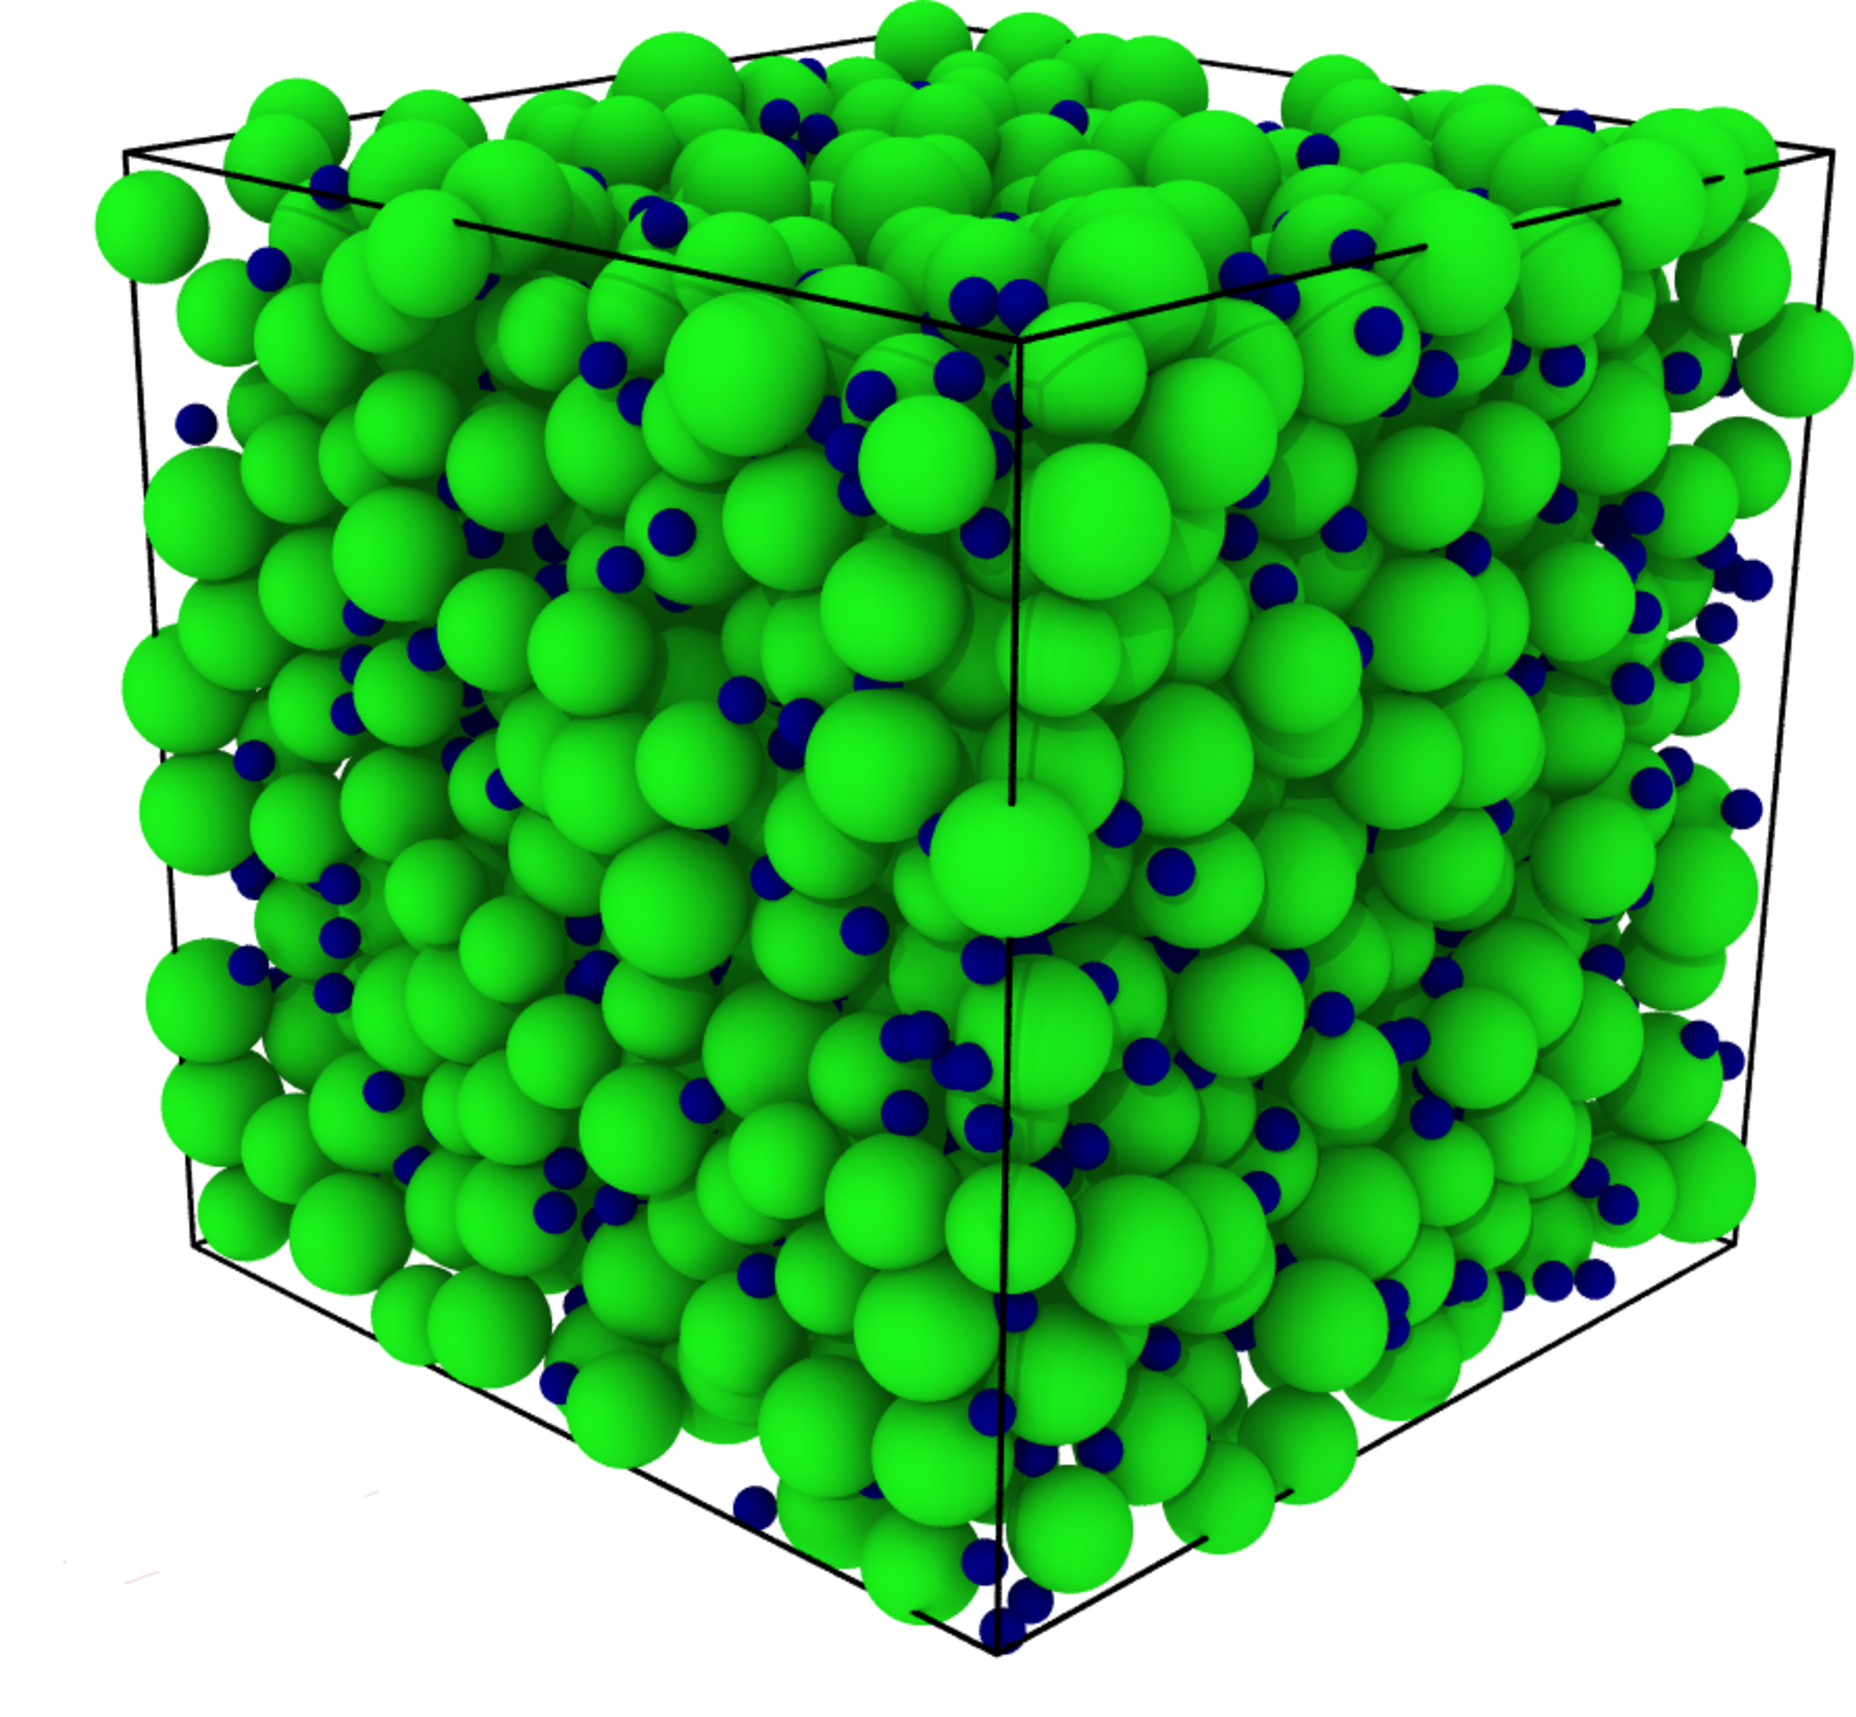
\includegraphics[width=12cm]{figs/fig6p1.pdf}
\caption[{\em Snapshot of the system at the density $\rho = 2.5$}]{Snapshot of the system at the density $\rho = 2.5$. A and
B particles are represented by green and dark blue spheres, respectively.
\label{fig6p1}}
\end{figure}
%%%%%%%

Using LAMMPS \cite{plimpton1995}, extensive molecular dynamics (MD) simulations are performed for systems with $N = 1000$, 2000, and 4000 particles, placed in a three-dimensional cubic box with periodic boundary conditions. Except otherwise stated, all reported results are for $N=2000$. The equations of motion are integrated using the velocity form of the Verlet algorithm \cite{allen2017} with a time step $dt = 0.00075 \, \tau_{\rm WCA}$.  The simulations are done for different number densities in the range $2.1 \le \rho \le 3.5$ at the temperature $T = 2/3$. For each density, 30 independent samples are simulated.  During the equilibration of the samples, the temperature is kept constant using a dissipative particle dynamics (DPD) thermostat \cite{soddemann2003} where the damping coefficient is set to 1.0. {Note that the DPD thermostat conserves linear momentum locally and thereby globally. And, we have chosen the damping coefficient such that the short-time dynamics under thermostatted conditions matches with the dynamics reported under microcanonical conditions \cite{horbach2009}. Furthermore, to obtain well-annealed samples at} the high densities, $\rho \ge 2.25$, the MD simulations are combined with the swap Monte Carlo (SMC) algorithm \cite{grigera2001, berthier2019}.  In a trial SMC move, one randomly selects a pair of particles, exchanges their diameters, and accepts or rejects this move according to a Metropolis criterion. In our scheme, only the diameters of the A particles are swapped. Every 100 MD steps, $N_{\rm A}$ trial SMC moves are done. The runs with the hybrid MD-SMC method were over $4 \times 10^8$ time steps for $\rho = 2.25$ and $6 \times 10^8$ time steps for $\rho \ge 2.296$. This is sufficient to fully equilibrate the system up to a density of 2.296. This we have checked by analyzing the decay of the incoherent intermediate scattering function (see below) in the presence of the SMC. Thus, the glass transition in our simulation occurs around $\rho_{\rm g} \approx 2.3$. For the MD production runs, the SMC is switched off, but they are performed with the coupling to the thermostat.

A snapshot of the system at the density $\rho = 2.5$ is shown in Fig.~\ref{fig6p1}. From this snapshot, one can infer that the large A particles form a close-packed structure while the small B particles can explore the free volume between the A particles.


We study the rheological behaviour of this model for the system consisting of $N = 2000$ particles. Initial states at different densities are sampled from our study on the quiescent behaviour. Apart from the 50:50 composition, we also study a couple of other compositions, viz.~100:0 and 75:25, in order to understand how the inclusion of B species changes the system's response to an external shear.

%
\begin{figure}[htb!]
\centering
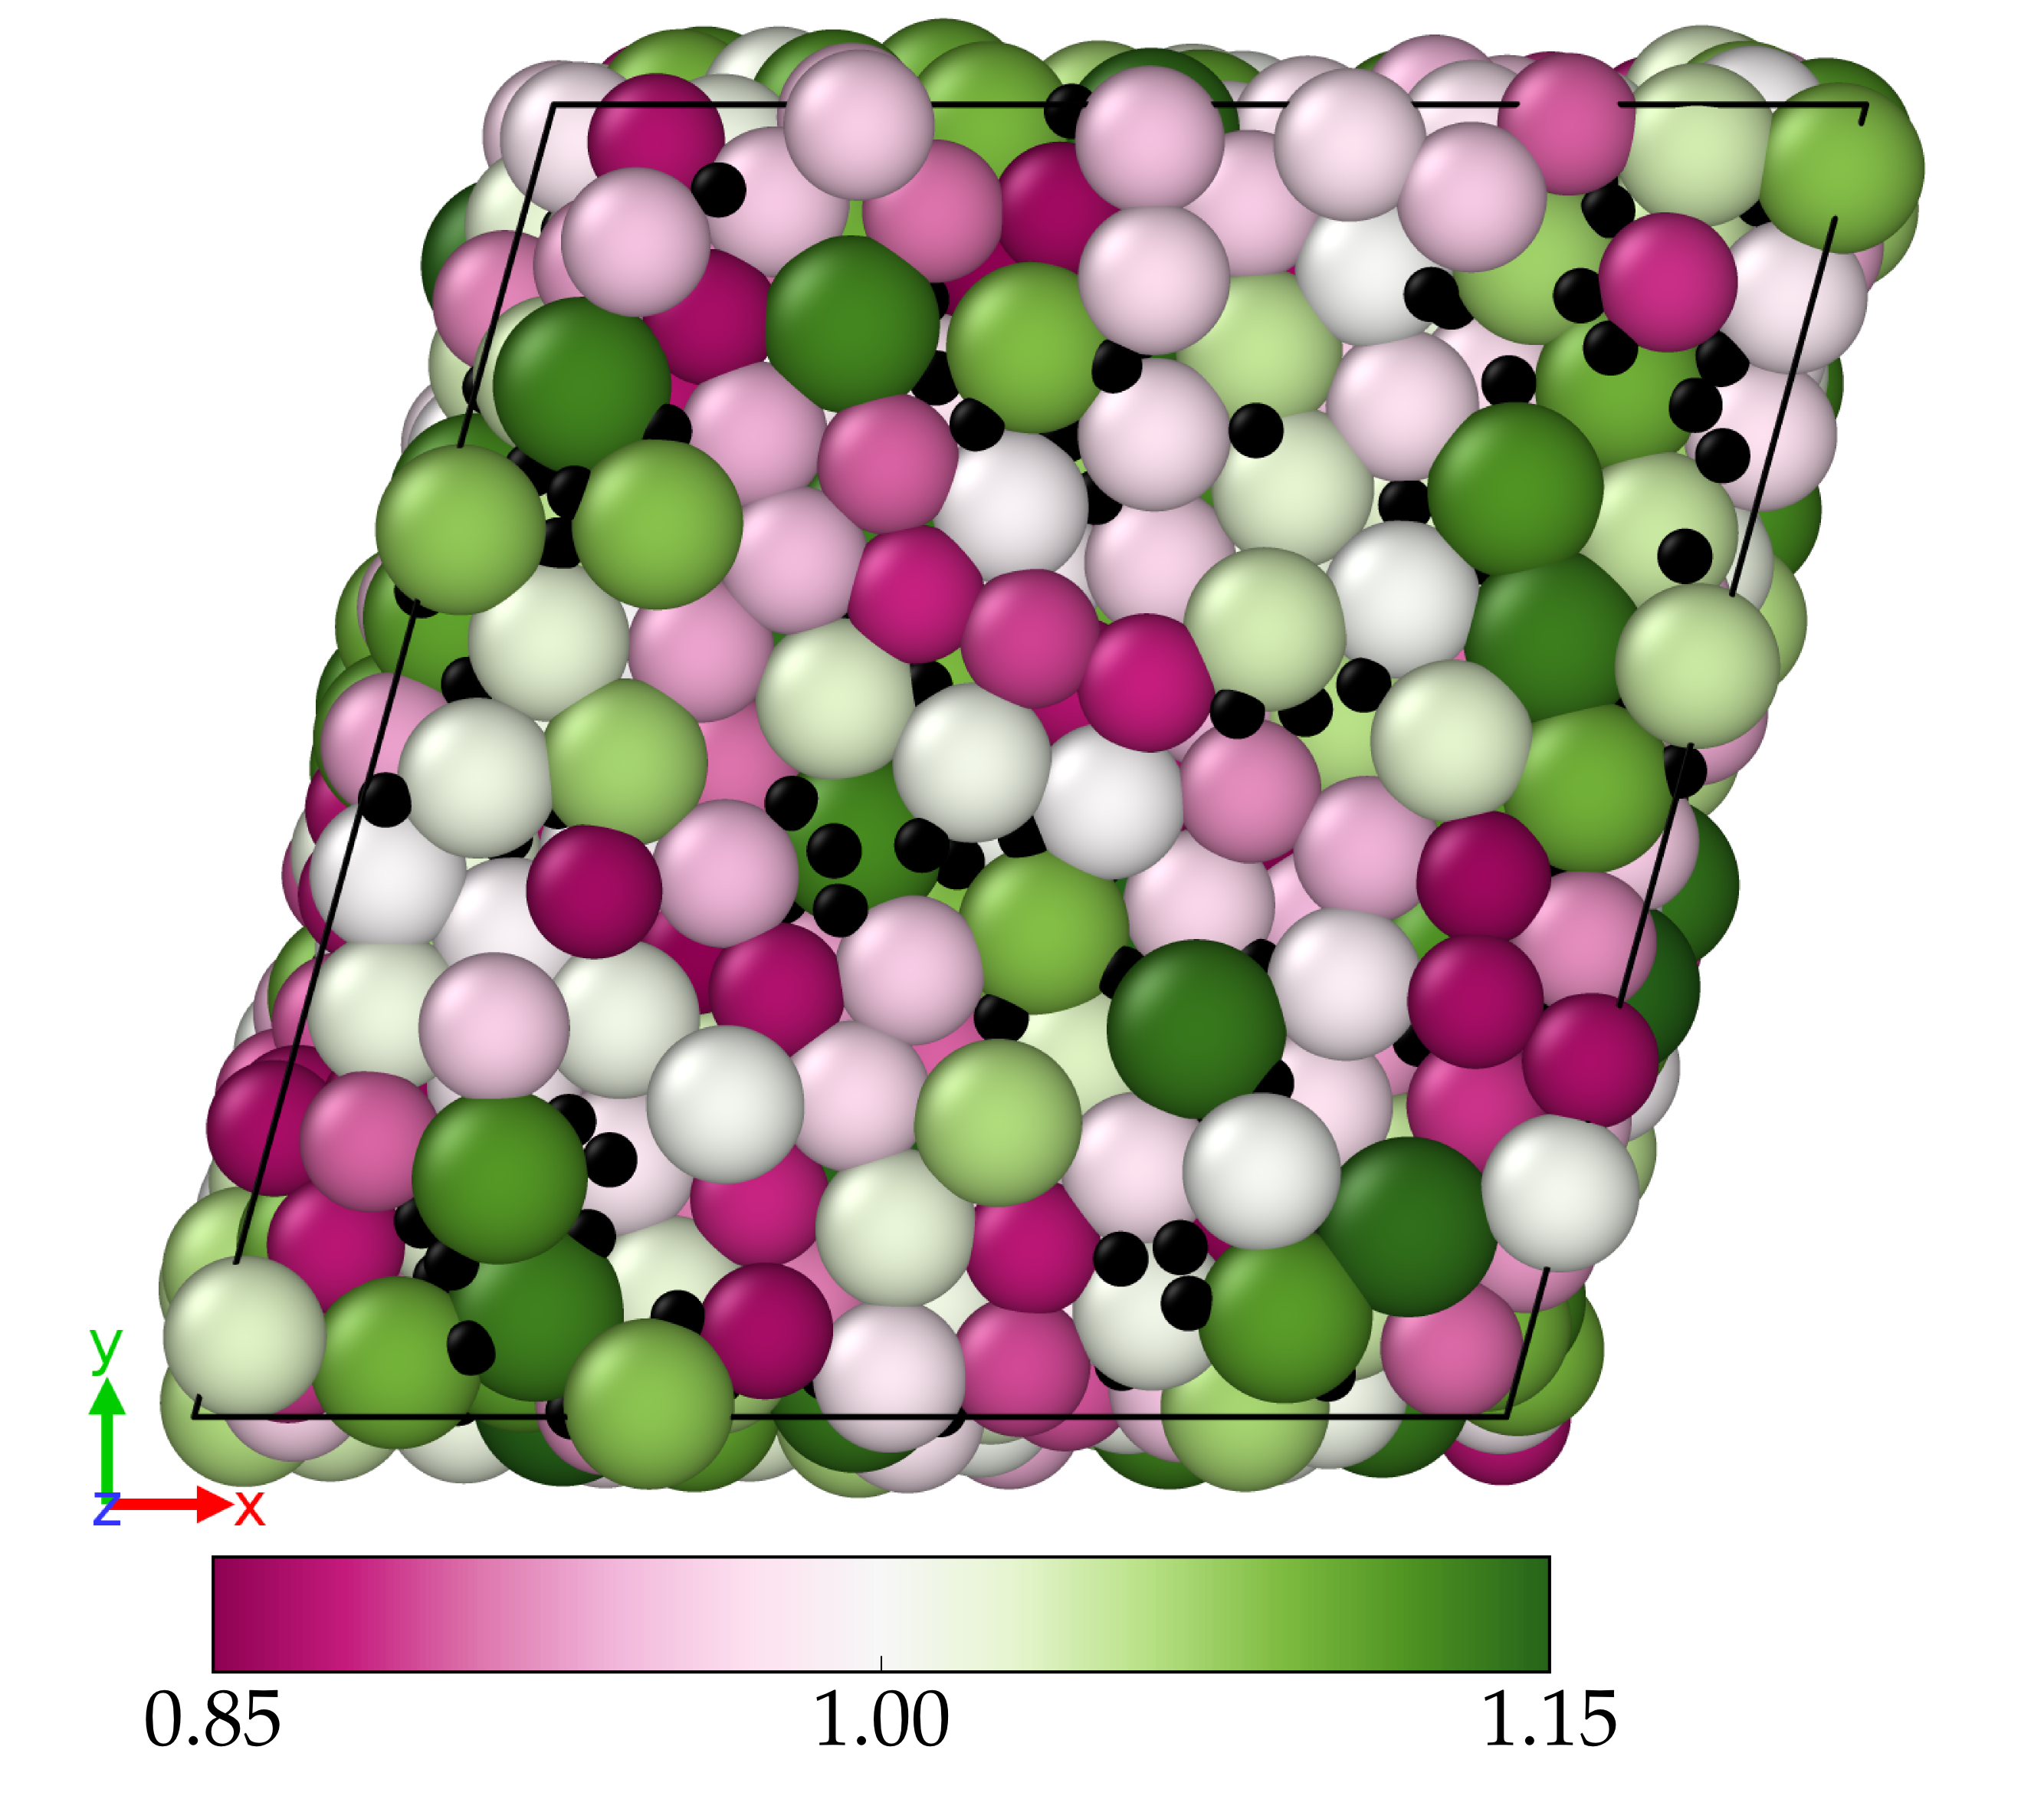
\includegraphics[width=12cm]{figs/fig7p1.png}
\caption{{\em Snapshot of the sheared binary mixture.} The color panel represents the diameter of the polydisperse larger species (A).  Smaller particles (B) are shown in black. The shear is applied in the $x$-direction along the $xy$ plane. 
\label{fig7p1}}
\end{figure}
%

To investigate the rheological response of the system, we impose shear along the $xy$ plane in the $x$-direction (see Fig.~\ref{fig7p1}) using different shear rates ($\dot{\gamma}$) ranging between $1.5{\times}10^{-6}$ and $10^{-3}$. Lees-Edwards boundary conditions are utilised during the shearing. The rheological behaviour is studied for a range of densities varying from very small, viz. $\rho_{\rm A}=1.05$ to very large $\rho_{\rm A}=1.75$, where $\rho_{\rm A}$ is the partial density of A species.  Note that all reported densities will be in terms of $\rho_A$, since we will be eventually probing how changing $\rho_{\rm B}$ influences the rheology at fixed $\rho_{\rm A}$, as discussed above. A snapshot of the sheared system is shown in Fig.~\ref{fig7p1}. As is evident, the larger species indeed populate most of the volume and the smaller species dot the intervening space. In this study, we inquire how the microscopic dynamics of these two species are manifested in the macro-rheology during the shear process.

%
\section{Results}

%%%%%%%%%%%%copied from JCP$$$$$$$$$$$$$$$$$$$$$$$$$$$$$$$$$$$$$$$$$$$$$$$$$$$$$$START

\subsection{Structural and dynamical properties in quiescence}
%
\subsubsection{Structural and thermodynamic properties}
%
With the aid of the SMC technique, we are able to obtain well-annealed samples at very high densities that are above the critical MCT density \cite{horbach2009} $\rho_c \approx 2.23$. However, at such high densities, one may expect that at least for the A particles, the thermodynamic equilibrium is an ordered crystalline phase. Although the large polydispersity of the A particles in our model suppresses crystallization to some extent, the use of the SMC technique tends to also accelerate the formation of crystalline clusters and therefore we check especially the high-density samples whether they are purely amorphous structures and thus free of any crystalline clusters. To this end, we measure static structure factors and analyse the samples in terms of local bond order parameters.  Furthermore, we determine the thermodynamic factor $\Phi$ from the concentration-concentration structure factor $S_{cc}(q)$.

The pressure $P$ increases monotonously with increasing density $\rho$ (Fig.~\ref{fig6p2}).  However, the lines connecting the points between $\rho = 2.25$ and $\rho = 2.296$ in $P(\rho)$ indicate a slight change of the slope (cf.~the inset of Fig.~\ref{fig6p2}). This could be due to a liquid-solid coexistence, occurring around these densities.  And indeed our analysis for the density $\rho = 2.296$ (see below) indicates the occurrence of crystalline clusters in some of the samples at that density.

\begin{figure}
\centering
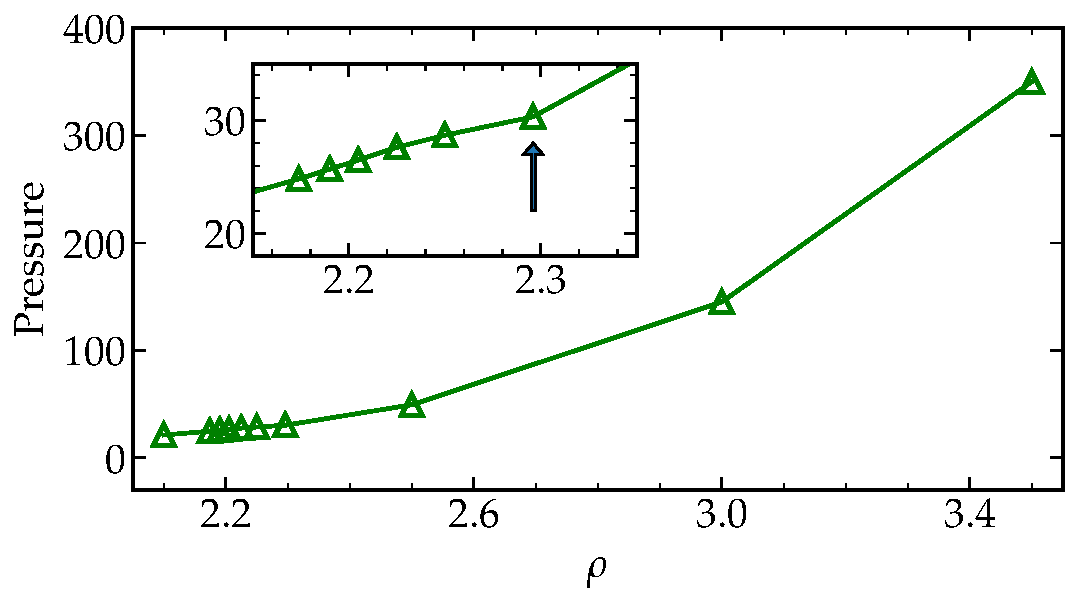
\includegraphics[width=15cm]{figs/fig6p2.pdf}
\caption[{\em Pressure $P$ as a function of density}]{Pressure $P$ as a function of density. The inset zooms in the region around $\rho = 2.296$ (this density is indicated by an arrow). 
\label{fig6p2}}
\end{figure}
%
\begin{figure}
\centering
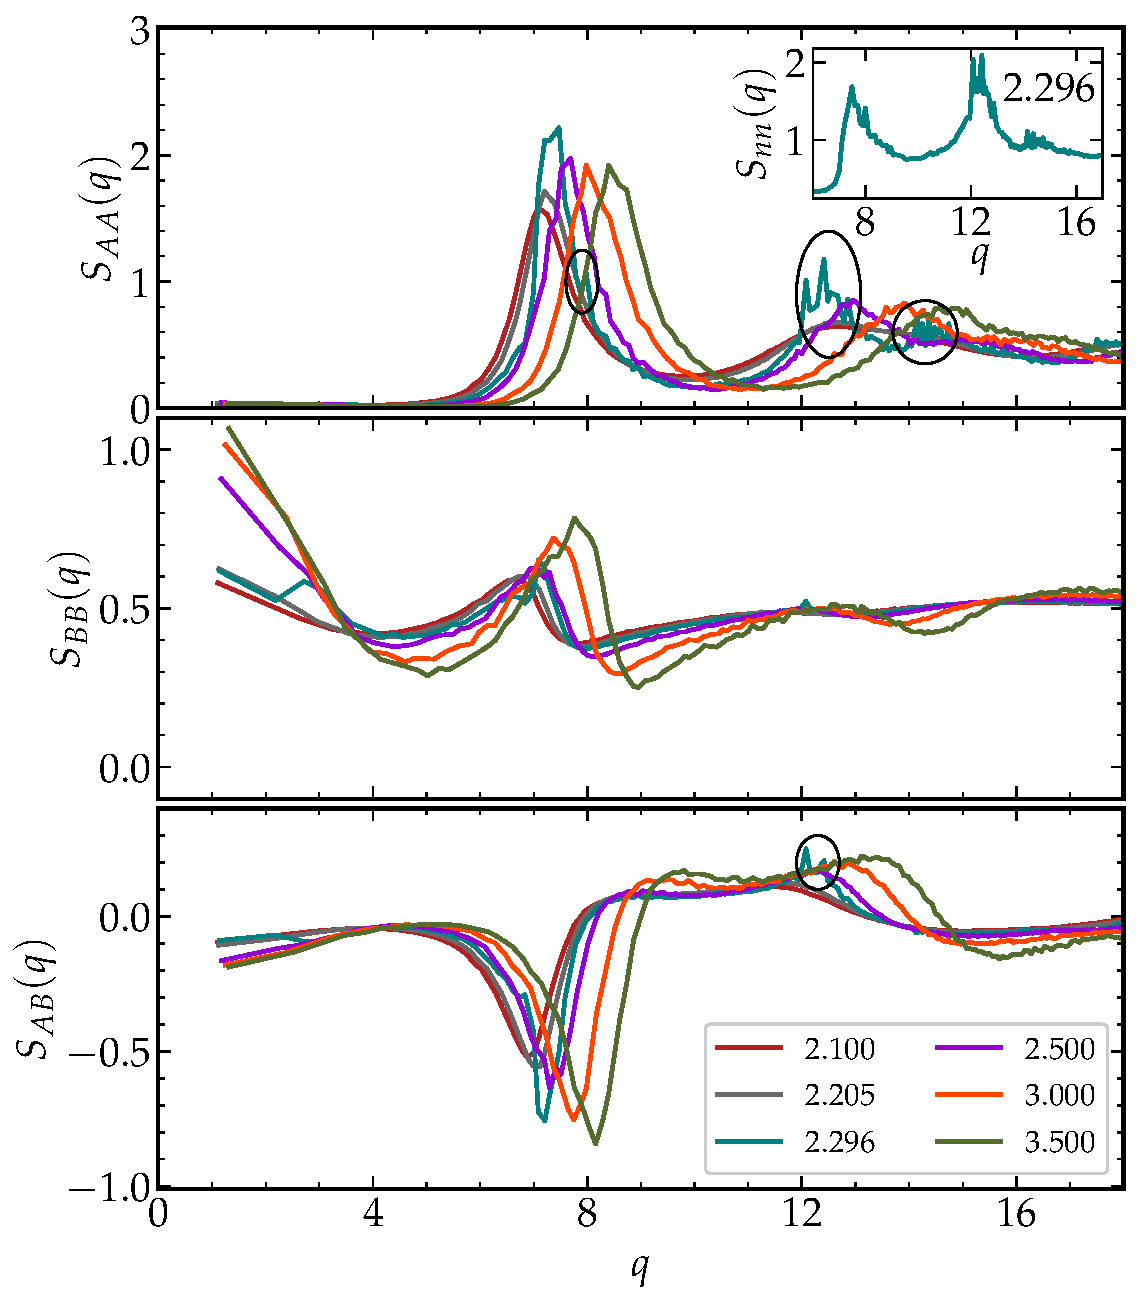
\includegraphics[width=10cm]{figs/fig6p3top.pdf}
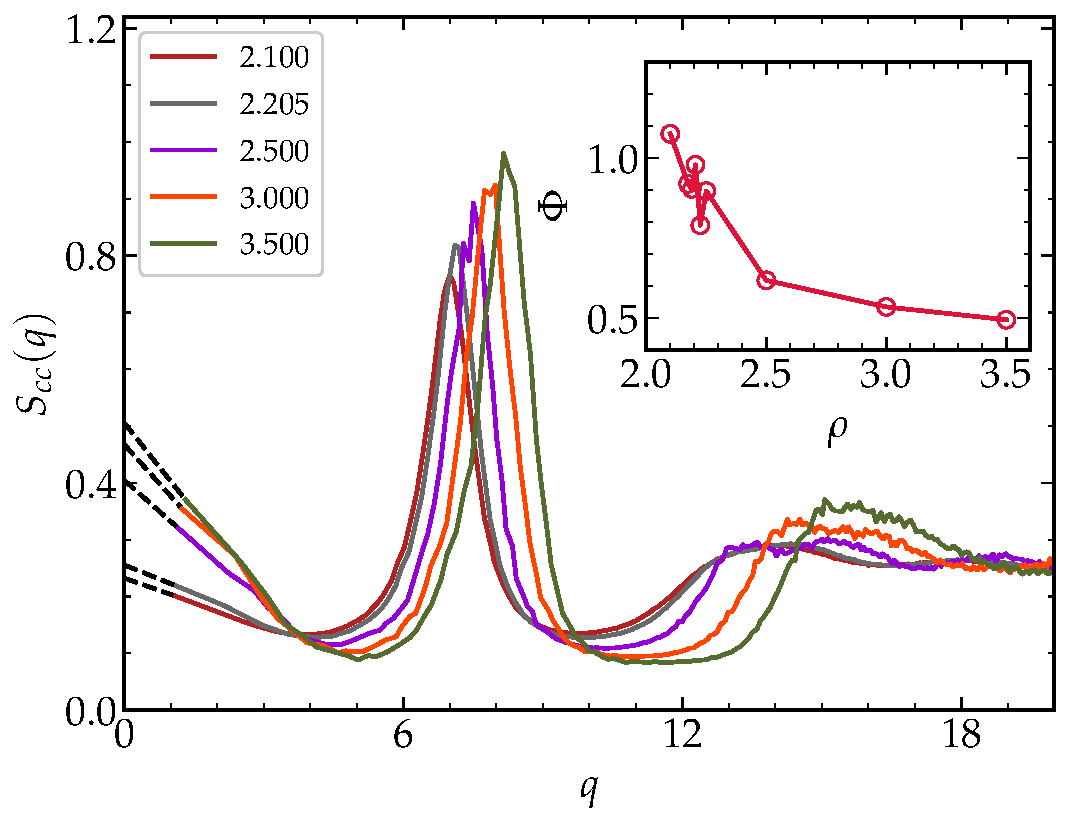
\includegraphics[width=10cm]{figs/fig6p3bottom.pdf}
\caption[{\em Partial structure factors and concentration-concentration structure factors $S_{cc}(q)$ at different densities. The thermodynamic factor $\Phi$, as obtained from the fit to $S_{cc}(q)$}]{{\bf Top panels:} Partial structure factors $S_{\rm AA}(q)$, $S_{\rm BB}(q)$, and $S_{\rm AB}(q)$ at different densities.  Emerging Bragg peaks are indicated by circles. The inset of the plot of $S_{\rm AA}(q)$ shows the total structure factor $S_{nn}(q)$ at the density $\rho = 2.296$. {\bf Bottom panel:} Concentration-concentration structure factor $S_{cc}(q)$ at different densities. The dashed lines indicate the extrapolation to $q=0$ via a fit function (see text). The thermodynamic factor $\Phi$, as obtained from the fitted $S(q=0)$, is shown in the inset as a function of density. \label{fig6p3}}
\end{figure}
%
%
\begin{figure}
\centering
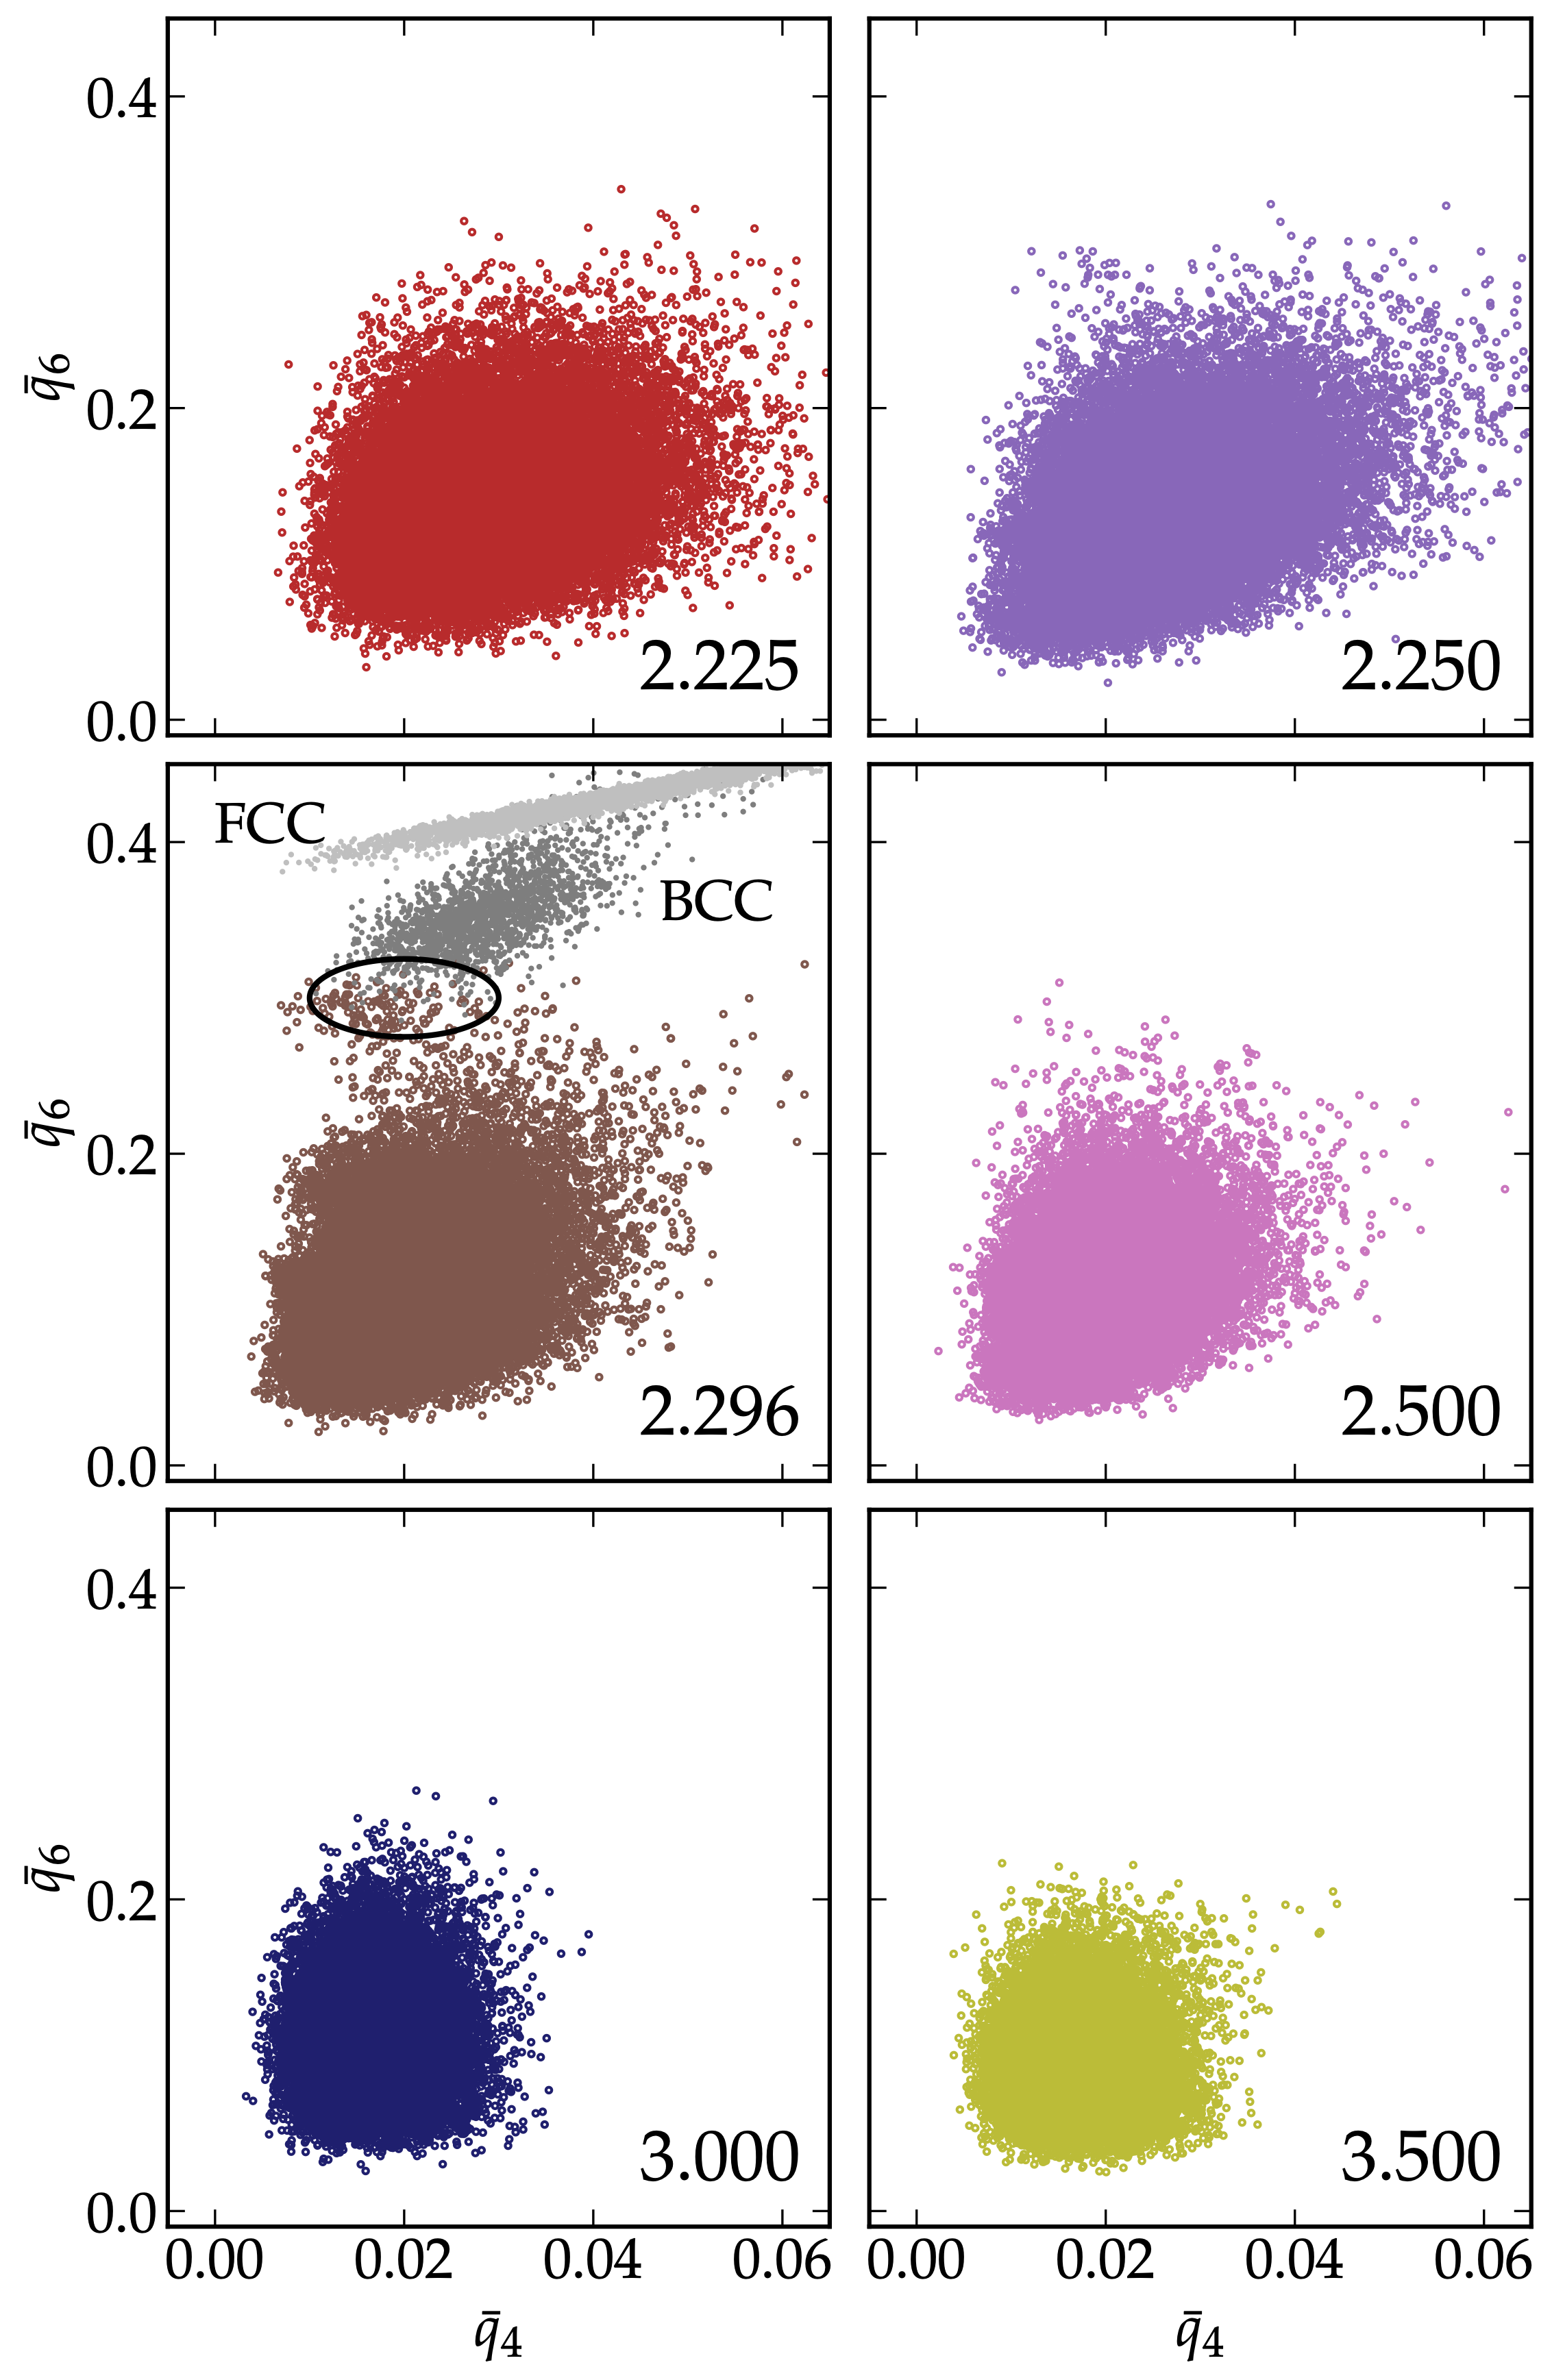
\includegraphics[width=13cm]{figs/fig6p4.png}
\caption[{\em Search for crystalline nuclei at different densities using $\bar{q}_4-\bar{q}_6$ analysis }]{$\bar{q}_4-\bar{q}_6$ plot for system at different marked densities (calculation with cutoff). {For density of $2.296$, scatters for thermalised BCC and FCC crystals are also marked (using dark gray and light gray colors). We also indicate the points where BCC crystallites are expected in our system (see text)}.\label{fig6p4}}
\end{figure}
%

To quantify the structural changes in our AB mixture with increasing density, we now consider the partial structure factors $S_{\alpha\beta}(q)$. The top panels of Fig.~\ref{fig6p3} show these functions for different values of $\rho$.  With increasing $\rho$, the first peak in both $S_{\rm AA}(q)$ and $S_{\rm BB}(q)$ shifts to larger $q$ as the inter-particle separation decreases. In between, at the density $\rho = 2.296$, $S_{\rm AA}(q)$ shows signatures of possible formation of local crystallites, with discrete spikes being clearly visible. Although less prominent, this is also reflected in the cross correlation, $S_{\rm AB}(q)$, as well as in the total structure factor $S_{nn}(q) = S_{\rm AA}(q) + S_{\rm BB}(q) + 2 S_{\rm AB}(q)$ that is shown in the inset of the plot of $S_{\rm AA}(q)$. However, for densities higher than $\rho = 2.296$ there is no sign of any Bragg peaks, suggesting that the samples at these high densities is purely amorphous. In fact, this is confirmed by our analysis of the samples in terms of local bond order parameters (see below).

In the bottom panel of Fig.~\ref{fig6p3}, we show how $S_{cc}(q)$ varies with increasing density. We extract $S_{\rm cc}(0)$ by extrapolating $S_{cc}(q)$ to $q = 0$, using the fit function $f(q) = S_{cc}(0) [1 - A\, q^2 + B\, q^4]$ (with $S_{cc}(0)$,$A$, and $B$ being fit parameters). For the fits (dashed lines), we have only taken into account the data for $q \le 2.0$. Then, from $S_{cc}(0)$ we compute the thermodynamic factor $\Phi$ via Eq.~(\ref{eq_phi}). The variation of  $\Phi$ is shown in the inset.  We observe that $\Phi$ decreases from a value of about 1.0 at $\rho = 2.1$ to a value of about 0.5 at the highest considered density, $\rho = 3.5$.  This rather weak variation of $\Phi$ over a broad range of densities also implies that the thermodynamic factor does not strongly affect the density dependence of the interdiffusion coefficient, which we discuss further below.



We have calculated the correlation between $\bar{q}_{4}$ and $\bar{q}_{6}$ for the A particles in our system (details regarding this analysis is discussed in section-\ref{structure} of Chapter-\ref{chap1}). The measured values of $\bar{q}_{4}$ and $\bar{q}_{6}$, for each particle across several representative configurations, can be visualized in the form of a scatter plot in the $\bar{q}_4$-$\bar{q}_6$ plane, following Ref.~\cite{dellago2008}, to check if local environments exhibit any formation of ordered structures. This is shown in Fig.~\ref{fig6p4}, for a few densities across the range that we have studied, using configurations sampled from $30$ independent trajectories. First thing to notice is that, across all the densities, the values of $\bar{q}_4$ are small ($<0.06$) and in fact shrink with increasing density. Similarly for $\bar{q}_6$, the numbers are in the liquid-like regime, except for $\rho=2.296$ where some pockets of BCC-like structures seem to be visible for some clusters within some trajectories. For reference, we also show in the same plot the scatters corresponding to equilibriated BCC and FCC structures at this density and temperature. Thereby, it indicates the presence of BCC crystallites in some of the configurations at this density, as also hinted by the partial structure factor analysis discussed above. 

To summarize, the structural changes with increasing density are on expected lines. There is some hint of occurrence of a small number of local crystallites, in the vicinity of the mode-coupling density. However, when supercooled to higher densities, the system remains disordered even when more annealed states are explored via SMC.

%
\subsubsection{Dynamical properties}
%
We will now discuss the dynamic properties of the mixture.  As mentioned earlier, for the model system that we are studying, the larger A species are known to exhibit a mode-coupling transition around \cite{horbach2009} $\rho_c \approx 2.23$. However, as pointed out earlier, this transition is avoided in reality; but, a glass transition of the A species is expected in the regime $\rho > \rho_c$. In the glassy regime, the A particles are expected to be in a frozen-in configuration on the diffusive time scale of the B particles.  However,  the diffusivity of the B particles also continues to decrease with increasing density such that they are expected to be in an arrested state at very large densities.

%
\begin{figure}
\centering
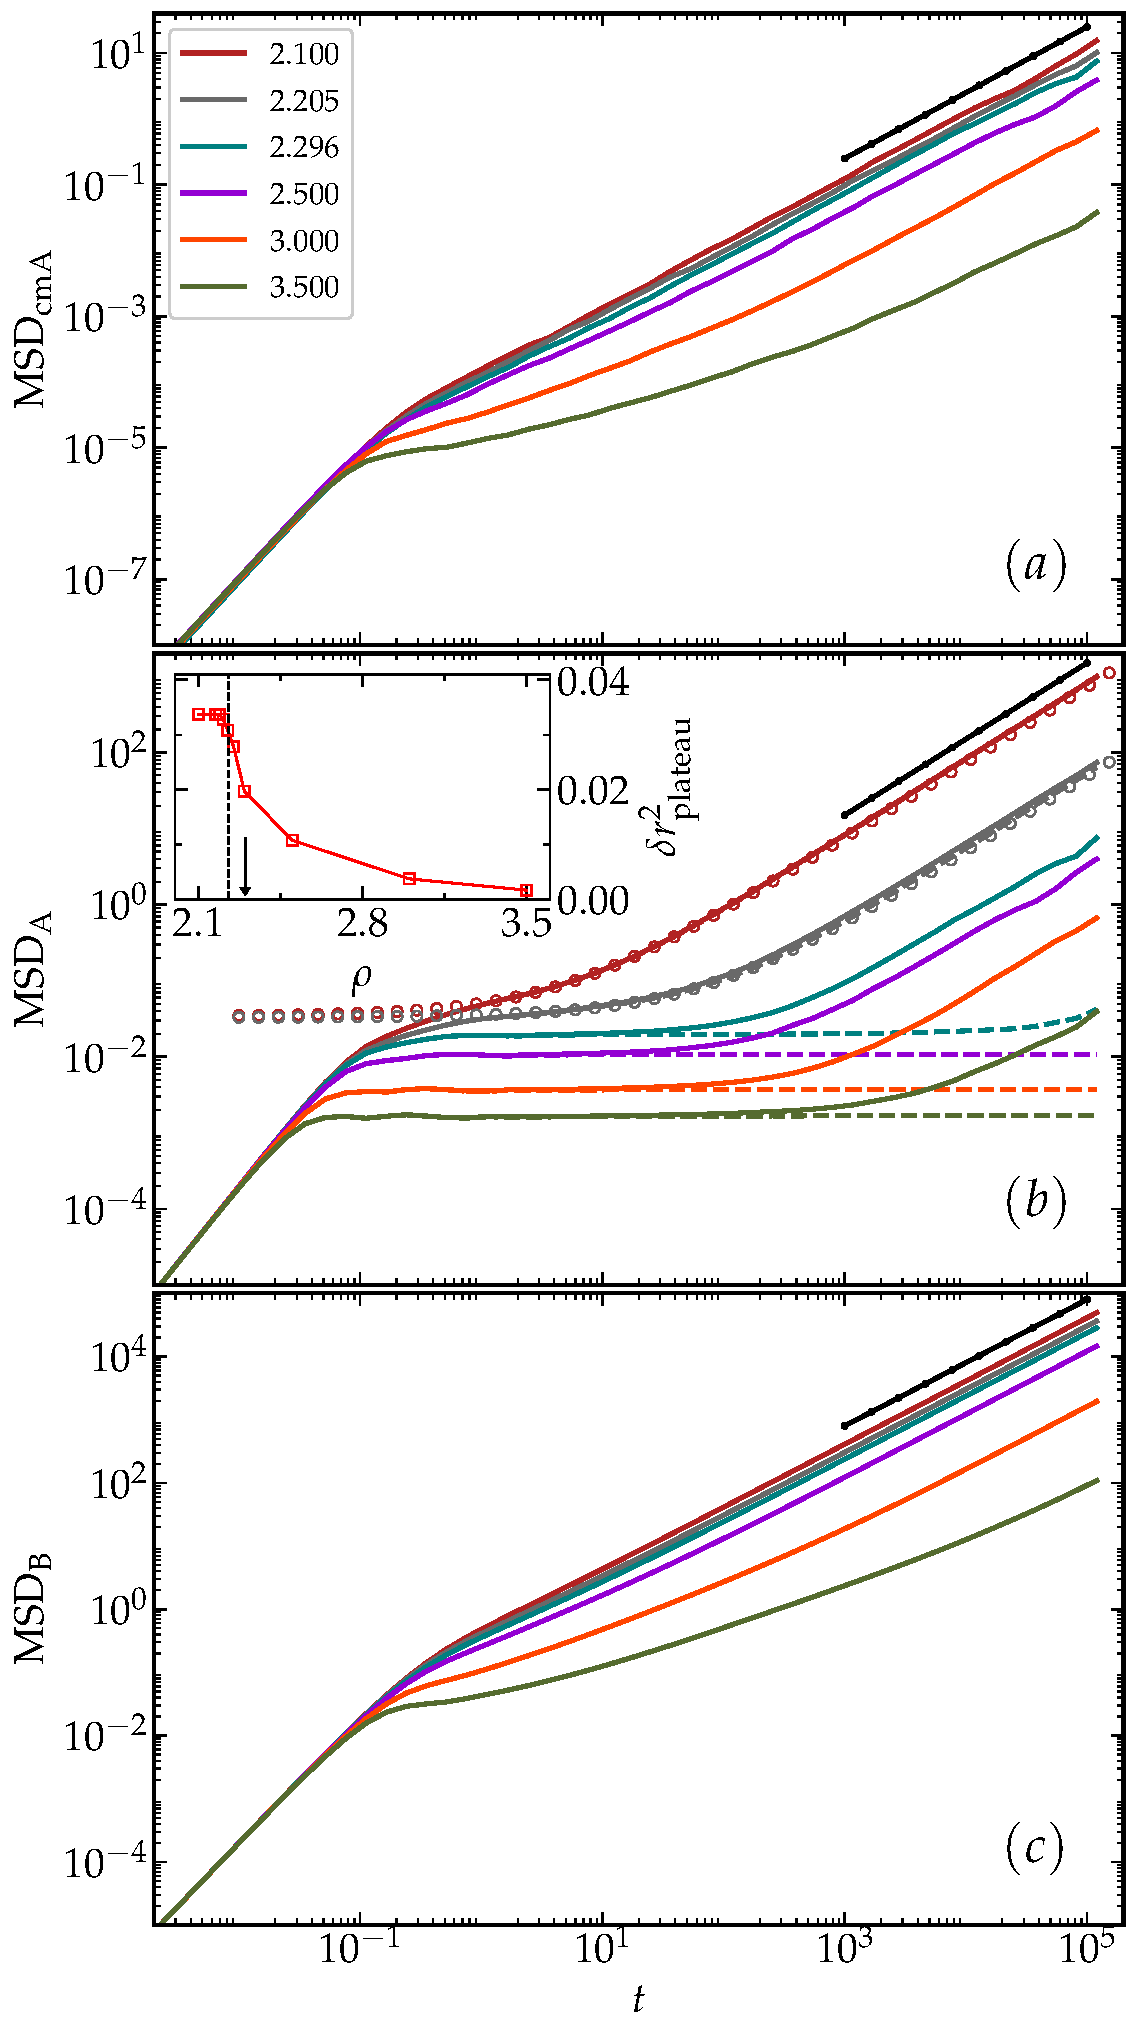
\includegraphics[width=10cm]{figs/fig6p5.pdf}
\caption[{\em Center-of-mass MSD and MSD of bigger and smaller species}]{(a) Center-of-mass MSD, {${\rm MSD}_{\rm cmA}(t)$, for different densities. (b) ${\rm MSD}_{\rm A}(t)$ and (c) ${\rm MSD}_{\rm B}(t)$} for the same densities. In (b) and (c), solid and dotted lines represent calculations with and without the center-of-mass correction, respectively (see text).  In all sub-plots, the solid lines with dots are straight lines $\propto t$ to indicate the diffusional regime of the MSDs at long times. {In (b), the open circles correspond to fits with Eq.~(\ref{eq_vs}). The inset in (b) shows the plateau height, $\delta r^2_{\rm plateau}$, as obtained from the fits with Eq.~(\ref{eq_vs}) as a function of density (here, the rectified ${\rm MSD}_{\rm A}(t)$'s from (b) are used). The vertical dashed black line marks the critical density $\rho_c = 2.23$; the glass transition density $\rho_{\rm g}\approx 2.3$ is marked by an arrow.}
\label{fig6p5}}
\end{figure}
%

%
\begin{figure}
\centering
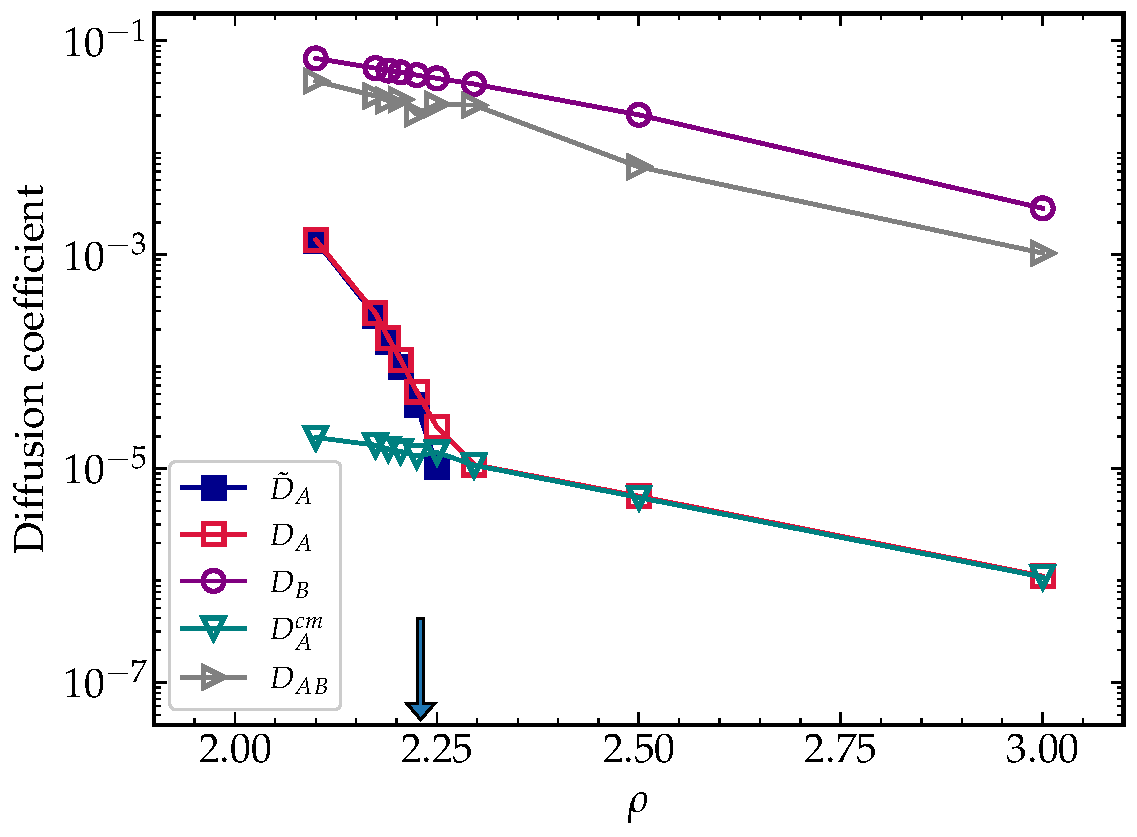
\includegraphics[width=13cm]{figs/fig6p6top.pdf}
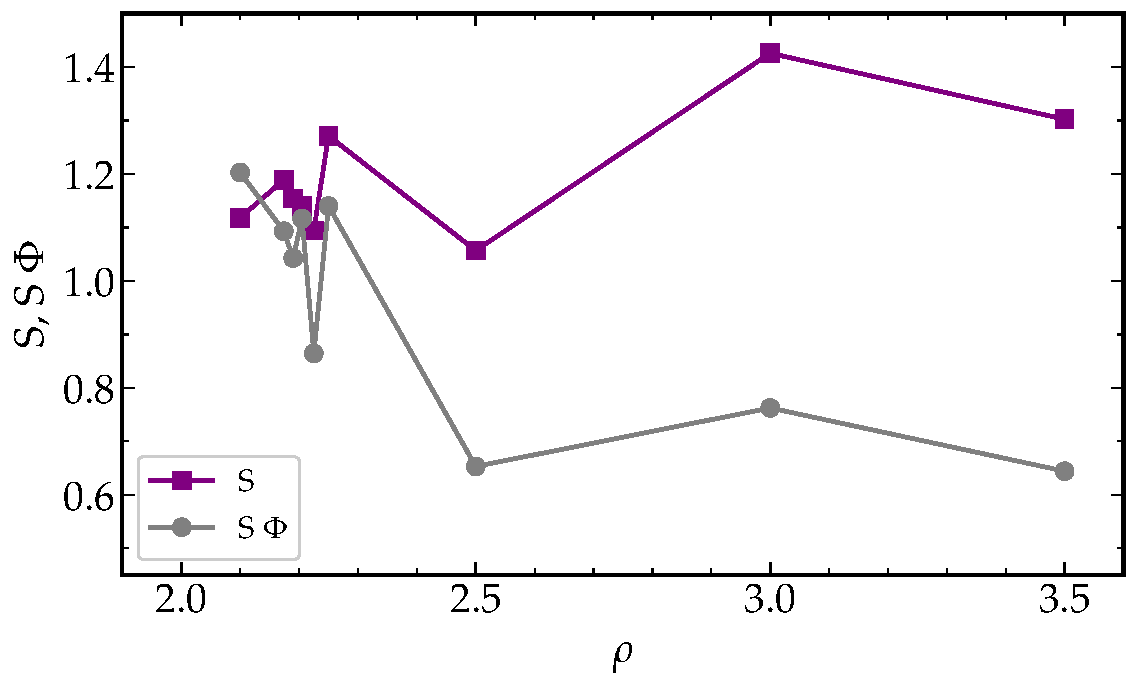
\includegraphics[width=13cm]{figs/fig6p6bottom.pdf}
\caption[{\em Variation of selfdiffusion coefficients, center-of-mass diffusion coefficient and interdiffusion coefficient with density. Manning factor ($S$) and the product $S \Phi$ as a function of density}]{{\bf Top panel:} Selfdiffusion coefficients $D_{\rm A}$ and $D_{\rm B}$, the center-of-mass diffusion coefficient $D_{\rm A}^{\rm cm}$  and the interdiffusion coefficient $D_{\rm AB}$ as a function of density $\rho$. Also shown is the rectified selfdiffusion coefficient $\tilde{D}_{\rm A}$ (see text). {The arrow} marks the previously estimated critical MCT density for $D_{\rm A}$ at $\rho_c=2.23$ \cite{horbach2009}.  {\bf Bottom panel:} Manning factor $S$ and the product $S \Phi$ as a function of density. \label{fig6p6}}
\end{figure}
%

In the following, our main objective is to study the density dependence of the interdiffusion coefficient. To this end, one has to monitor the trajectory of the center of mass of the A species and the corresponding time evolution of {${\rm MSD}_{\rm cmA}(t)$}, as defined by Eq.~(\ref{eq_msdcm}), needs to be computed.  This MSD is shown in Fig.~\ref{fig6p5}a for different densities.  For the same densities, Figs.~\ref{fig6p5}b and \ref{fig6p5}c display the single-particle MSDs, {${\rm MSD}_\alpha (t)$} (see Eq.~(\ref{eq_msd})), of the A and B particles, respectively.  For the A species, {${\rm MSD}_{\rm A}$} shows the behaviour that is expected for a typical glassforming liquid. There is a short-time ballistic regime ($\propto t^2$) and a long-time diffusive regime ($\propto t$). In between these two regimes, there is a plateau-like region that becomes more pronounced and broader with increasing density. The latter regime is due to the intermediate caging of the particles. Importantly, we note that even for $\rho > \rho_c$, the MSD of A particles still displays diffusive dynamics at long times. Below, we show that this feature is a finite-size effect, i.e.~the observed diffusive regime for $\rho > \rho_c$ shifts to longer time scales with increasing system size. {The shape of ${\rm MSD}_{\rm B}$ for the B species} is very different from that of the A particles, with no intermediate plateau at all. We will also discuss this, below.  Now, if we look at the MSD curves for the center-of-mass motion, it is evident that they bear close resemblance with that of the B species, the reason for which will be evident once we analyse the diffusion coefficients.


The long-time dynamical behaviour is well characterized by measuring the respective diffusion coefficients, measured from the corresponding MSD data.  The density variation of the measured single-particle diffusion coefficients, $D_{\rm A}$ and $D_{\rm B}$, the center-of-mass diffusion coefficient $D_{\rm A}^{\rm cm}$ as well as the interdiffusion coefficient $D_{\rm AB}$ are shown in top panel of Fig.~\ref{fig6p6}.  First, we note that the diffusion coefficient of the smaller B particles remains finite beyond $\rho_c$ (indicated via the arrow), consistent with previous study \cite{horbach2009}.  Now, if we look at the data for $D_{\rm A}$, we observe that it decreases as it approaches $\rho_c$, as reported earlier, and beyond that there seems to be a separate branch of weaker decrease with density. Interestingly, for $\rho > \rho_c$, the measured center-of-mass diffusion coefficient,  $D_{\rm A}^{\rm cm}$, shows exactly the same density dependence.  As already noted in the previous paragraph, the measured interdiffusion coefficient has a density dependence which resembles that of the diffusivity of B species, over the entire density range.

We now analyse the motion of A particles for $\rho > \rho_c$. Since the density dependence of $D_{\rm A}$, in this density regime, matches that of $D_{\rm A}^{\rm cm}$, it implies that the observed motion of the individual A particles is actually due to the motion of the center of mass of the A species.  To disentangle that, we compute the MSD of the A particles by shifting to the frame of reference of the population's center of mass i.e., $\vec{r}^{\; \prime {\rm \; (A)}}_j(t) = \vec{r}_j^{\rm \; (A)}(t) - \vec{R}_{\rm A}(t)$. The redefined MSDs are plotted in the top panel of Fig.~\ref{fig6p5}, using dashed lines. We observe that following this rectification, there is a significant change in the MSD in the large density regime. The rectified MSDs, in that regime, exhibit a prolonged plateau over the time window of our observation implying that in the frame of reference of the center of mass, the particles are essentially caged and there is hardly any cage-breaking, especially for $\rho \geq 2.5$. Therefore, we can conclude that only due to the motion of the center of mass, deviations from the plateau are exhibited in the bare MSDs at these densities. At small enough density ($\rho=2.1$), this rectification is not observed, and there is a mild rectification for $\rho=2.205$.  The rectified selfdiffusion coefficient of the A particles is also shown in Fig.~\ref{fig6p6}, from which it is evident that the rectified $D_{\rm A}$, labelled as $\tilde{D}_{\rm A}$, sharply decreases around $\rho_c$. Thus, the apparent kink in the density dependence of $D_{\rm A}$ is a consequence of the crossing of $\tilde{D}_{\rm A}(\rho)$ and $D_{\rm A}^{\rm cm}$.

As discussed above, the emergence of a plateau in ${\rm MSD}_{\rm A}$ indicates the caging of the A particles. A prediction of MCT, describing the initial increase of the MSD from the plateau towards the diffusive regime, is given by the following function \cite{goetze2009},
%
\begin{equation}
\Phi(t) =  \delta r^2_{\rm plateau} + h t^b + h_2 t^{2b} \, ,
\label{eq_vs}
\end{equation}
%
with $\delta r^2_{\rm plateau}$ the height of the plateau, $h$ and $h_2$ density-dependent amplitudes, and $b$ a critical exponent. Fits with Eq.~(\ref{eq_vs}) are shown in Fig.~\ref{fig6p5}(b) (with open circles). Here, $\delta r^2_{\rm plateau}$, $h$, and $h_2$ are used as fit parameters and the exponent is fixed to $b=0.5$. Note that the fits are done for densities up to $2.25$ and for densities above this, plateau heights are just read off from the MSD measurements. In the large density regime, the rectified mean squared displacement data are used for this analysis. The inset in Fig.~\ref{fig6p5}(b) displays the resulting plateau height $\delta r^2_{\rm plateau}$ as a function of density. Around the critical density $\rho_c$ (marked as a vertical line in the inset), one can infer a change in the behavior of $\delta r^2_{\rm plateau}$. While below $\rho_c$ the extracted plateau height is a constant, $\delta r^2_c \approx 0.033$, it decreases with increasing density above $\rho_c$. The kink seen at $\rho\approx 2.3$ can be identified as the location of the glass transition density where the system falls out of equilibrium. The constant $\delta r^2_c$ for $\rho < \rho_c$ marks the stability limit of the amorphous solid state \cite{goetze2009, fuchs1998, lamp2022}. It is related to a critical localization length, $\xi_c = \sqrt{\delta r^2_c /6} \approx 0.074$. Dividing $\xi_c$ by the typical nearest neighbor distance $d$ between A particles, one obtains $\xi_c/d \approx 0.07$ (here, $d=1.0588$ is used, corresponding to the location of the first peak of the radial distribution function for the AA correlations at $\rho=2.1$). With respect to the A species, this value of $\xi_c/d$ can be interpreted as the Lindemann criterion for the amorphous solid stability of our system (see also Ref.~\cite{lamp2022}).

%
\begin{figure}
\centering
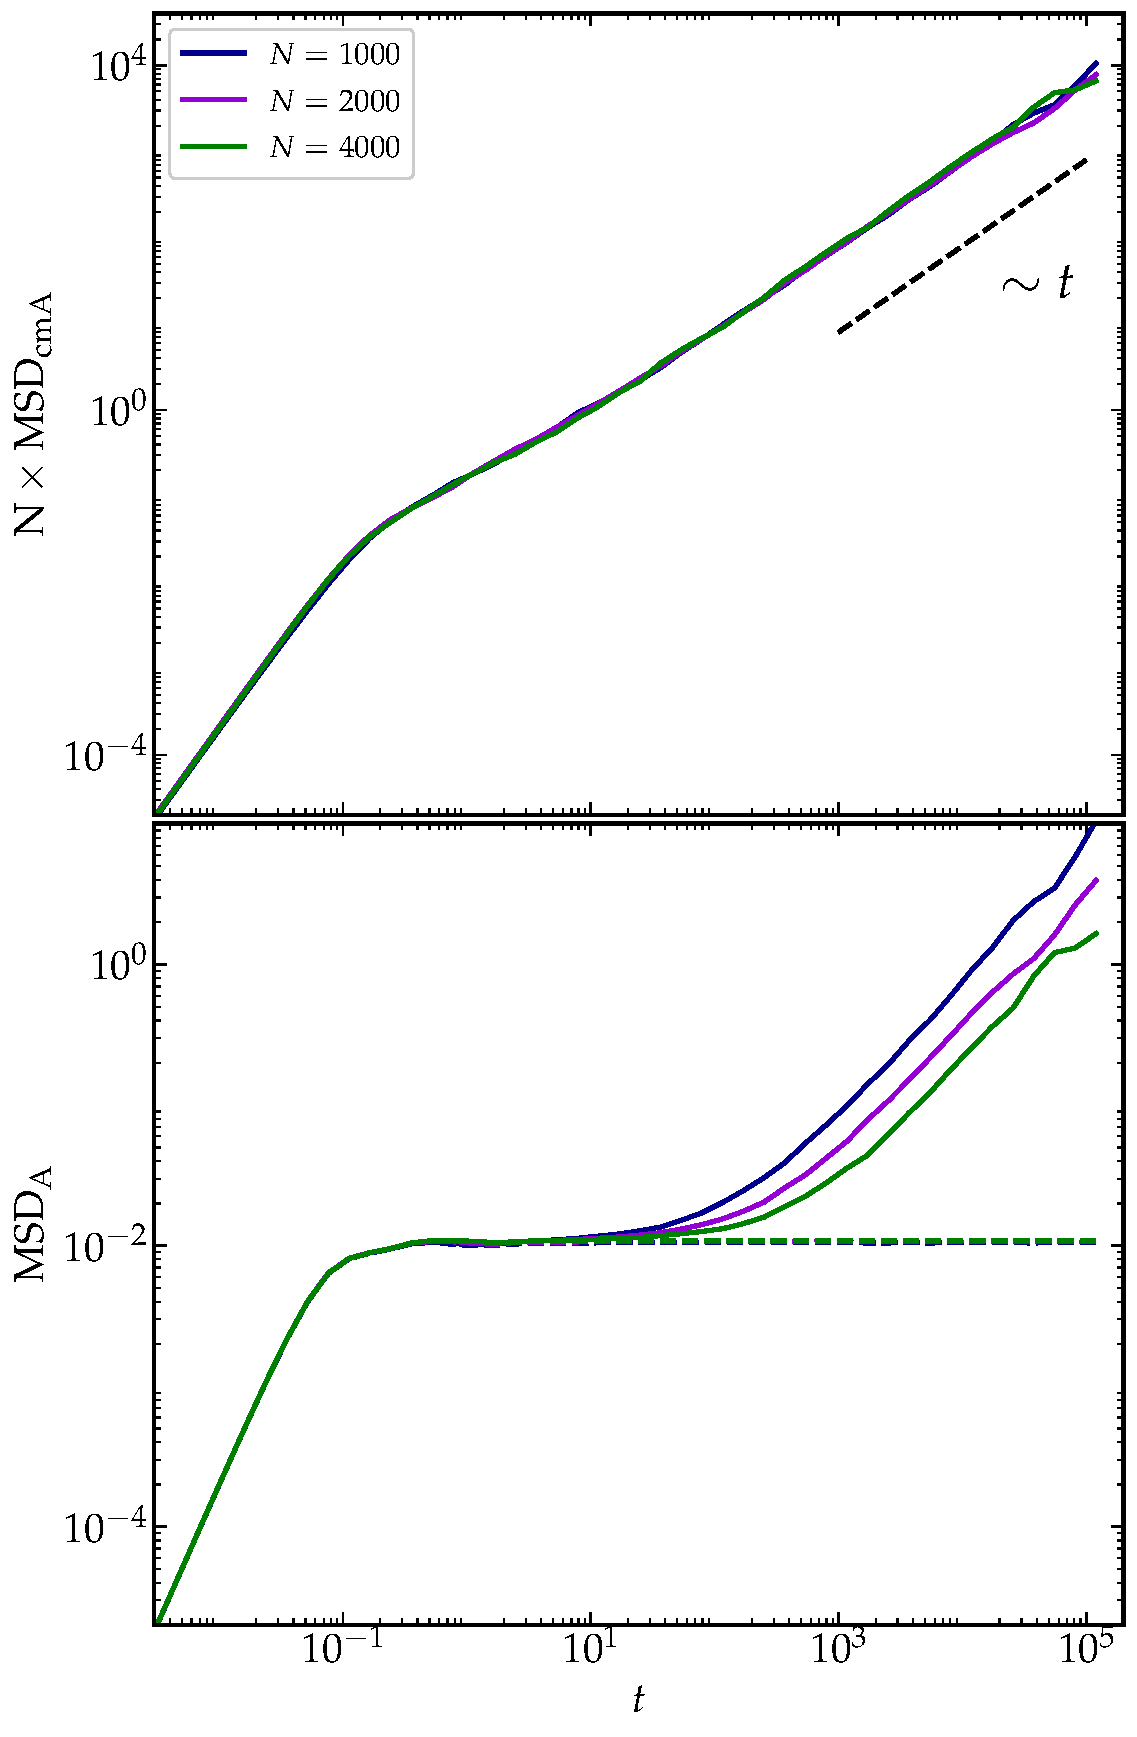
\includegraphics[width=13cm]{figs/fig6p7.pdf}
\caption[{\em Center-of-mass MSD for A species, scaled with system size and single particle MSD of the A species at the same density, for the different system sizes}]{{\bf Top panel:} Center-of-mass MSD for A species, scaled with system size $N$, at density $\rho=2.5$. {\bf Bottom panel:}  Single particle MSD of the A species at the same density, for the different system sizes. Solid and dotted lines represent calculations without and with center-of-mass correction, respectively.
\label{fig6p7}}
\end{figure}
%

Having clarified the actual density dependence of $D_{\rm A}$, we can now use Eq.~(\ref{eq_dabdarken}) to analyse the behaviour of the interdiffusion coefficient. If the Manning factor is $S=1.0$, Eq.~(\ref{eq_dabdarken}) reduces to the Darken equation (\ref{eq_darken}). Then, when $D_{\rm A}=0$, $D_{\rm AB} \sim D_{\rm B}$, which explains the observed behaviour of the interdiffusion coefficient in the regime $\rho \gg \rho_c$.  Physically, even though there is a dynamical arrest of the A species, because of momentum conservation, the mobility of B species leads to the center-of-mass motion of the A species and the consequent finite interdiffusion coefficient. We also note that even at lower densities, $D_{\rm B} > D_{\rm A}$, and thus there too, the behaviour of $D_{\rm AB}$ is also dependent on the diffusive motion of the smaller but faster B particles.

Furthermore, we test the validity of the Darken approximation for the mixture that we are studying. To do that, we consider two different quantities, viz $S=D_{\rm AB}/(x_{\rm A} D_{\rm B} + x_{\rm B} D_{\rm A})$ and $S\Phi$, which are plotted in the bottom panel of Fig.~\ref{fig6p6}. If the Darken approximation works, then $S$ should be around 1. As we can infer from Fig.~\ref{fig6p6}, over the whole range of densities, both $S$ and $S \Phi$ deviate from unity by less than a factor of 2, while the interdiffusion coefficient decreases by about two orders of magnitude.  So neither the cross correlations nor the thermodynamic factor strongly affect the density dependence of $D_{\rm AB}$ which is therefore essentially given by the linear combination of selfdiffusion coefficients, i.e.~$D_{\rm AB} \approx 0.5 (D_{\rm A} + D_{\rm B}$).


In the above discussions, we have noted that the MSD curves for B species do not show any plateau-like feature, i.e.~the absence of any signatures of caging by neighbouring particles. Rather, these curves show anomalous intermediate subdiffusive dynamics prior to diffusion. This is similar to what is observed in the case of interacting particles moving in a quenched environment of soft obstacles \cite{schnyder2018, schnyder2015}. For the binary mixture that we are studying, this is a reasonable scenario considering the large size ratio (see Fig.~\ref{fig6p1} for the visualisation). At the large density beyond $\rho_c$ where we are probing the dynamics, the A population is nearly frozen, and the B particles are diffusing through this quenched environment with which they interact via some soft interaction. For the case of interacting particles moving in a quenched environment of soft obstacles, an avoided localization transition is observed \cite{schnyder2018}, and one would expect a similar situation for the eventual dynamical arrest of the B species at large enough densities \cite{horbach2009}.


Next, we analyse the finite size effects in the measured diffusivities. Since the interdiffusion coefficient can be written as $D_{\rm AB} = \Phi L$, where $L = N D_{\rm A}^{\rm cm}$, as discussed in the previous section, $D_{\rm AB}$ has no finite size effects. This is illustrated in the top panel of Fig.~\ref{fig6p7}, where we plot the center-of-mass MSD of A species scaled with system size, at density of $\rho=2.5$, for a density larger than $\rho_c$. We observe that the curves for the different system sizes collapse for the scaled MSD, implying that ${N}D_{\rm A}^{\rm cm}$ is the same and therefore $D_{\rm AB}$ remains unaffected. On the other hand, the bare single particle MSDs show system size dependence at the same density, as shown in the bottom panel of Fig.~\ref{fig6p7}. However, if we now measure the MSD of the particles in the frame of reference of the center of mass of the A particles, as defined above, we observe that all collapse on the same plateau; see bottom panel of Fig.~\ref{fig6p7}.  This implies, that the finite size dependence in the single particle dynamics is coming from the change in centre-of-mass motion. However, as discussed above, this effect gets scaled out when computing the interdiffusion coefficient. {Furthermore, it is also evident that since $D_{\rm A}^{\rm cm}$ decreases with increasing $N$, the apparent kink in $D_{\rm A}(\rho)$ will shift to larger densities, with the shift depending on the sharpness via which $\tilde{D}_{\rm A}(\rho)$ vanishes.} For smaller $N$, the location of this apparent kink will similarly shift to smaller densities. Therefore the kink's location, which has a geometric origin, is  unrelated to where the dynamical transition happens.


%%%%%%%%%%%%copied from JCP$$$$$$$$$$$$$$$$$$$$$$$$$$$$$$$$$$$$$$$$$$$$$$$$$$$$$$END
\begin{figure}[htb!]
    \centering
	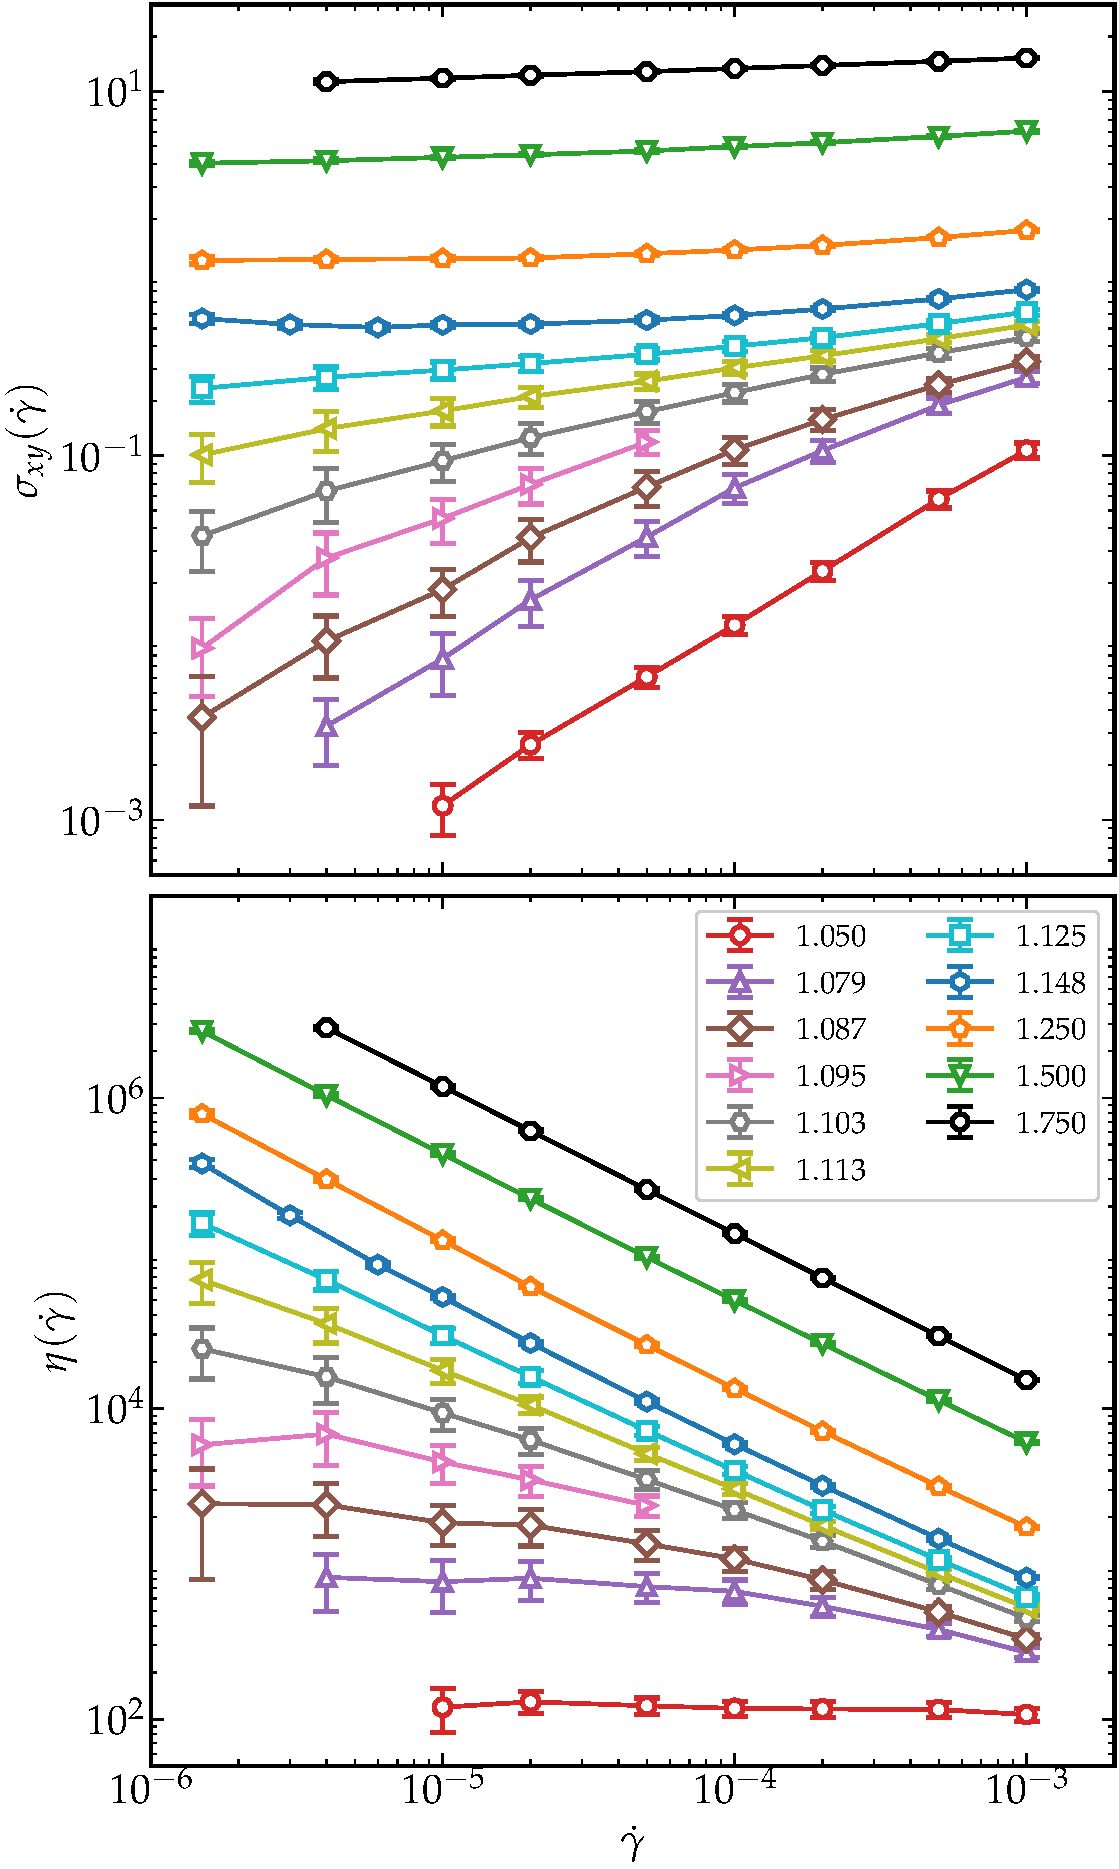
\includegraphics[width=12cm]{figs/fig7p3.pdf}
	\caption[{\em Variation of steady-state shear stress and corresponding viscosity with applied shear rate}]{{\em Rheological response.} Variation of steady-state shear stress $\sigma_{xy}$ (top) and corresponding viscosity $\eta$ (bottom) with applied shear rate $\dot{\gamma}$, at different partial densities ($\rho_{\rm A}$) of bigger species as marked. 
\label{fig7p3}}
\end{figure}
%

%

\subsection{Rheological response}

\subsubsection{Steady-state macroscopic shear response}
%
Next, we discuss the rheological response of the system over a range of densities and shear rates. A snapshot of the system during shear is shown in Fig.~\ref{fig7p1}, with the large size disparity of the two species distinctly visible.

Since the shear is imposed along the $xy$ plane, we measure the corresponding shear stress $\sigma_{xy}$ using the following Irving-Kirkwood expression: $\sigma_{xy} = \langle \frac{1}{V} \sum_{\alpha\beta} f^{x}_{\alpha\beta} r^{y} \rangle$, where $f^{x}_{\alpha\beta}$ is the $x$-component of the force with respect to a pair of particles and $r^y$ is the $y$-component of the distance vector between two particles labelled $\alpha$ and $\beta$ which could belong to either of the species A and B. $V$ is the total volume of the simulated system.  $\langle\cdot\rangle$ corresponds to averaging over states sampled in steady state.

At each density and imposed shear rate, we obtain the steady state by shearing the system to large strains and then ensuring that the measured shear stress $\sigma_{xy}$ fluctuates around a steady mean value. The data gathered for the variation of shear stress with imposed shear rate, i.e., the flow curve, for the wide range of densities is shown in the top panel of Fig.~\ref{fig7p3}. And, the corresponding viscosity defined by $\eta (\dot{\gamma}) = \sigma_{xy}(\dot{\gamma})/\dot{\gamma}$ is shown in the bottom panel of Fig.~\ref{fig7p3}.

%
\begin{figure}[htb!]
	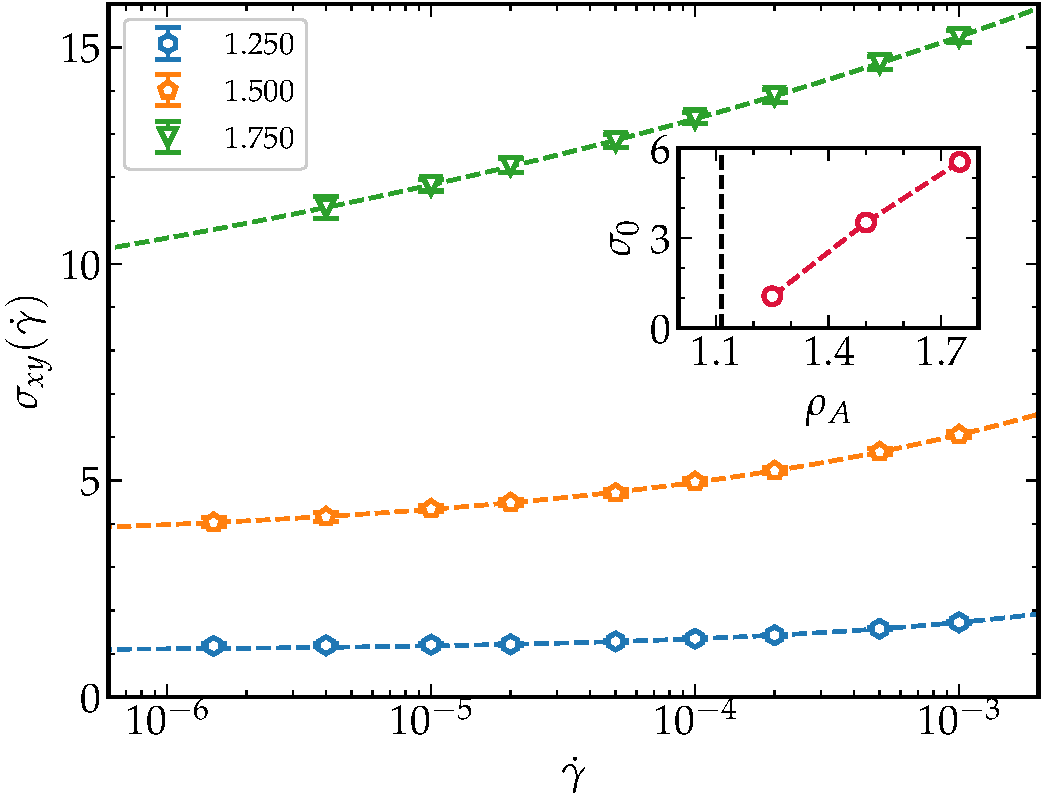
\includegraphics[width=14cm]{figs/fig7p4.pdf}
	\centering
	\caption[{\em Herschel-Bulkley fits to estimate the value of yield stress}]{{\em Herschel-Bulkley fits.} Flow curves, i.e., shear stress vs.~strain-rate at different partial densities ($\rho_{\rm A}$) of bigger species as marked, shown with corresponding Herschel-Bulkley fit ($\sigma = \sigma_0+K\dot{\gamma}^n$) using dotted line. Fit estimates are $\sigma_0 = 1.06, 3.52, 5.54$, $K = 8.33, 13.92, 18.63$ and $n = 0.36, 0.25, 0.09$ for $\rho_{\rm A} = 1.25, 1.50, 1.75$. (Inset) Variation of estimated value of yield stress $\sigma_0$ with $\rho_{\rm A}$. Dotted vertical line marks $\rho_{\rm A}^{\rm MCT}$. \label{fig4}}
\end{figure}
%

The main findings from the rheological data are the following. At small densities ($\rho_{\rm A} < 1.09$), a Newtonian regime, i.e., $\eta (\dot{\gamma})$ is constant, is observed at small shear rates. At larger shear rates, shear thinning is observed, i.e., the viscosity decreases with increasing $\dot{\gamma}$. The Newtonian regime shrinks with increasing density, i.e., pushed to smaller and smaller shear rates. These are distinct characteristics of complex liquids. As the density is increased, an apparent yield stress becomes visible at $\rho_{\rm A} \approx 1.125$, with $\sigma_{xy}$ becoming flat with decreasing $\dot{\gamma}$. This implies that there is an onset of macroscopic rigidity for the binary mixture. Around this density regime, there is also a change in behaviour of $\eta (\dot{\gamma})$ with shear-rate -- in the window of small shear rates, the viscosity continues to be an increasing function with decreasing $\dot{\gamma}$, i.e., there is no tendency to change curvature towards plateauing out. With further increase of density, the apparent yield stress of the system, viz.~$\sigma_{xy}(\dot{\gamma} \rightarrow 0)$, increases steadily, which is characteristic to amorphous solids. Note that the flow curve for $\rho_A = 1.148$ is slightly non-monotonic at small shear rate, the physical origin of which is uncertain and needs further investigation.

One can fit the variation of stress with shear rate in the large density regime using the Herschel-Bulkley (HB) function, $\sigma = \sigma_0+K\dot{\gamma}^n$, where $\sigma_0$ is the estimated yield stress, $K$ is a constant and $n$ is the HB exponent. The fits to the measured data for different $\rho_{\rm A}$ are shown in Fig.~\ref{fig4} and the values of the fit parameters are listed in the caption. In the inset of Fig.~\ref{fig4}, we display the emergence and increase of the estimated yield stress $\sigma_0$ with density, beyond $\rho_{\rm A}^{\rm MCT}$ .

%
\begin{figure}[htb!]
\centering
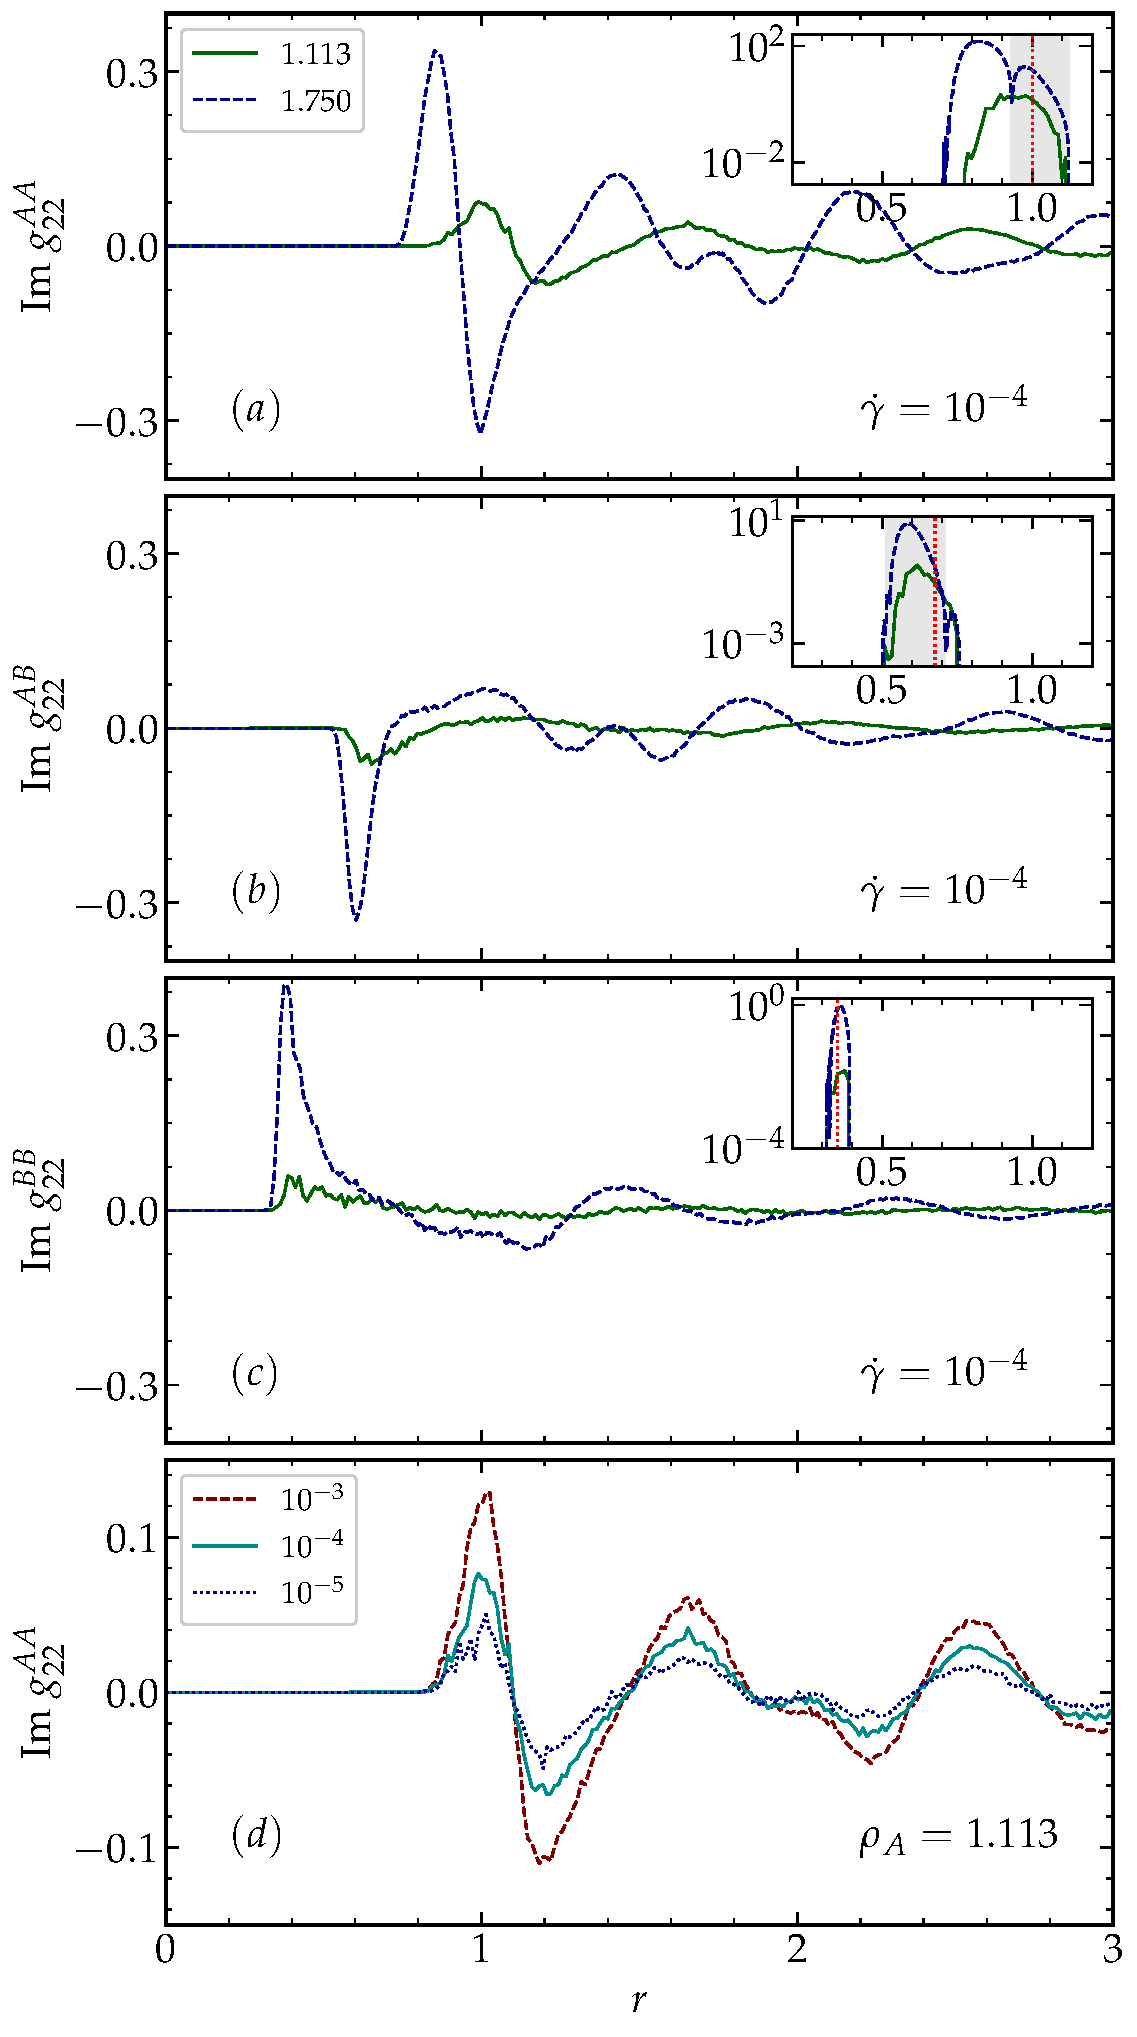
\includegraphics[width=10cm]{figs/fig7p5.pdf}
\caption[{\em Structural analysis in the sheared steady state using $g_{22}^{\alpha \beta}(r)$}]{{\em Structural analysis in the sheared steady state.} (a-c) The functions ${\rm Im}\, g_{22}^{\alpha \beta}(r)$ (see text for definition) at $\dot{\gamma} = 10^{-4}$ for the partial densities $\rho_{\rm A} = 1.113$ (solid line) and $\rho_{\rm A} = 1.75$ (dashed line). The corresponding insets show the absolute value of the integrand ${\rm I}^{\alpha\beta}(r)$ (see text). Here, the shaded area marks the range for which ${\rm I}^{\alpha\beta}(r)$ is negative at the partial density $\rho_{\rm A} = 1.75$. The red vertical dashed line marks the distance corresponding to the cutoff radius of the pair potential $V^{\alpha\beta}$ (see text) (d) Spatial variation of ${\rm Im} \, g_{22}^{\rm AA}(r)$ at $\rho_{\rm A} = 1.113$ for three different shear rates $10^{-3}, 10^{-4}$ and $10^{-5}$.} \label{fig5} 
\end{figure}
%

Overall, on a qualitative level, such variation of rheological flow curves, viz.~the emergence of a yield stress with the variation in a control parameter (e.g.~temperature or packing fraction or density) are very similar to the ones obtained in other soft-sphere glassy systems \cite{ludovic2002, sollich2012, sollich2013, golkia2020, lamp2022}. However, it would be interesting to quantify how the structural interplay between the glassy A particles and the mobile B particles contribute to the total stress $\sigma_{xy}$ and thus to the behavior of the flow curve. In this context, it also desirable to obtain spatial information about the structural anisotropies due to shear. To address all these issues, it is useful to consider the expansion of the partial radial distribution functions $g^{\alpha\beta}(r)$ ($\alpha\beta = {\rm AA, AB, BB}$) into spherical harmonics $Y_{lm}(\theta, \phi)$ of degree $l$ and order $m$, depending on the spherical coordinates $\theta$ and $\phi$ \cite{hanley1987, rainwater1988, gan1992}. This expansion reads
%
\begin{equation}
  g^{\alpha \beta}(r) = \sum_{l=0}^{\infty} \sum_{m=-l}^{l} 
  g^{\alpha\beta}_{lm}(r) Y_{lm}(\theta, \phi) \, . 
\end{equation}
%
Note that for an isotropic system only the coefficient $g_{00}^{\alpha\beta}(r)$ gives a non-vanishing contribution.

In our case of shear in a simple Couette flow geometry, the imaginary part of the coefficient with $l=2$ and $m=2$, ${\rm Im} \, g_{22}^{\alpha\beta}(r)$, is of particular importance since it gives the largest anisotropic correction to $g_{00}^{\alpha\beta}(r)$. Moreover, the shear stress can be computed from the functions ${\rm Im} g_{22}^{\alpha\beta}(r)$ using
%
\begin{equation}
\sigma_{xy} = \sigma_{xy}^{\rm AA} + \sigma_{xy}^{\rm BB} + \sigma_{xy}^{\rm AB}
\label{eq_sigmag22}
\end{equation}
%
where
%
\begin{eqnarray}
\sigma_{xy}^{\alpha \beta} & = & 
\int_0^\infty dr \; {\rm I}^{\alpha\beta}(r) \quad {\rm with} \\
{\rm I}^{\alpha\beta} & = & - f_1 \rho^2 \sqrt{2\pi/15} c_{\alpha} c_{\beta} r^3 \frac{\partial V^{\alpha\beta}(r)}{\partial r}  {\rm Im} \, g_{22}^{\alpha\beta}(r) \, .
\label{eq_integrand}
\end{eqnarray}
%
Here, $c_{\alpha} = N_{\alpha}/N$ and $f_1 = 1$ if $\alpha = \beta$ else $f_1 = 2$, and $V^{\alpha\beta}(r)$ is the potential between a pair of particles, separated by a distance $r$. The function ${\rm Im} \, g_{22}^{\alpha\beta}(r)$ can be expressed as
%
\begin{equation}
{\rm Im} \, g_{22}^{\alpha \beta}(r) = f \biggl< \sum_{i}^{N_{\alpha}} \sum_{j (\neq i)}^{N_{\beta}} \delta(|{\bf r}_i^{\alpha} - {\bf r}_j^{\beta}| - r) \frac{(x_i^{\alpha}-x_j^{\beta})(y_i^{\alpha}-y_j^{\beta})}{(r_i^{\alpha}-r_j^{\beta})^4} \biggl>.
\label{eq_img22}
\end{equation}
%
Here, $f = \sqrt{15}N/(\sqrt{8\pi} \rho N_{\alpha}N_{\beta})$, $\alpha\beta \in \{A,B\}$ and $\bf{r}_i^{\alpha}$ is the position vector of the $i$th particle of type $\alpha$.

Figures \ref{fig5}(a) to \ref{fig5}(c) respectively show the functions ${\rm Im} g_{22}^{\alpha\beta}(r)$ for the AA, AB, and BB correlations, in each case at the shear rate $\dot{\gamma} = 10^{-4}$ for $\rho_{\rm A}=1.113$ (in the fluid regime) and $\rho_{\rm A} = 1.75$ (in the yield stress regime). The insets display the corresponding absolute values of the integrands $\rm I^{\alpha\beta}(r)$, as defined by Eq.~(\ref{eq_integrand}). Here, the shaded area marks the region where the integrand is negative for the partial density $\rho_{\rm A} = 1.75$. As we can infer from the plots, the contribution $\sigma_{xy}^{\rm AB}$ to the total stress is negative. However, the main contribution to the total stress, and therefore to the eventual macroscopic rigidity, is due to the AA correlations. This contribution is positive and about one order of magnitude larger than that due to the AB correlations and two orders of magnitude larger than that due to the BB correlations. Note that the correlations increase with increasing density, which leads to larger stresses. In the insets of Figs.~\ref{fig5}(a) -(c), we have also marked as red vertical dashed lines the location of the cutoff radius of the pair potential $V^{\alpha\beta}$  which is $1.00$, $(1.00+0.35)/2$ and $0.35$ for AA, AB and BB pairs, respectively. Note that due to the polydispersity of the A species, the cutoff radius is different for each pair of A particles and so the indicated radius 1.00 corresponds to an average cutoff radius. However, with this choice, we obtain the total shear stress via Eqs.~(\ref{eq_sigmag22}-\ref{eq_img22}), in agreement with the stress, as directly computed from the Irving-Kirkwood expression.

The variation of correlations with shear-rate is illustrated in Figure \ref{fig5}(d), where we show ${\rm Im} \, g_{22}^{\rm AA}(r)$ at $\rho_{\rm A} = 1.113$ for the three different shear rates $10^{-3}$, $10^{-4}$, and $10^{-5}$. The decrease of the amplitude of the peaks in this function with decreasing shear rate is reflected in a decrease of the shear stress with decreasing shear rate (cf.~Fig.~\ref{fig7p3}).

%
\begin{figure*}[htb!]
\centering
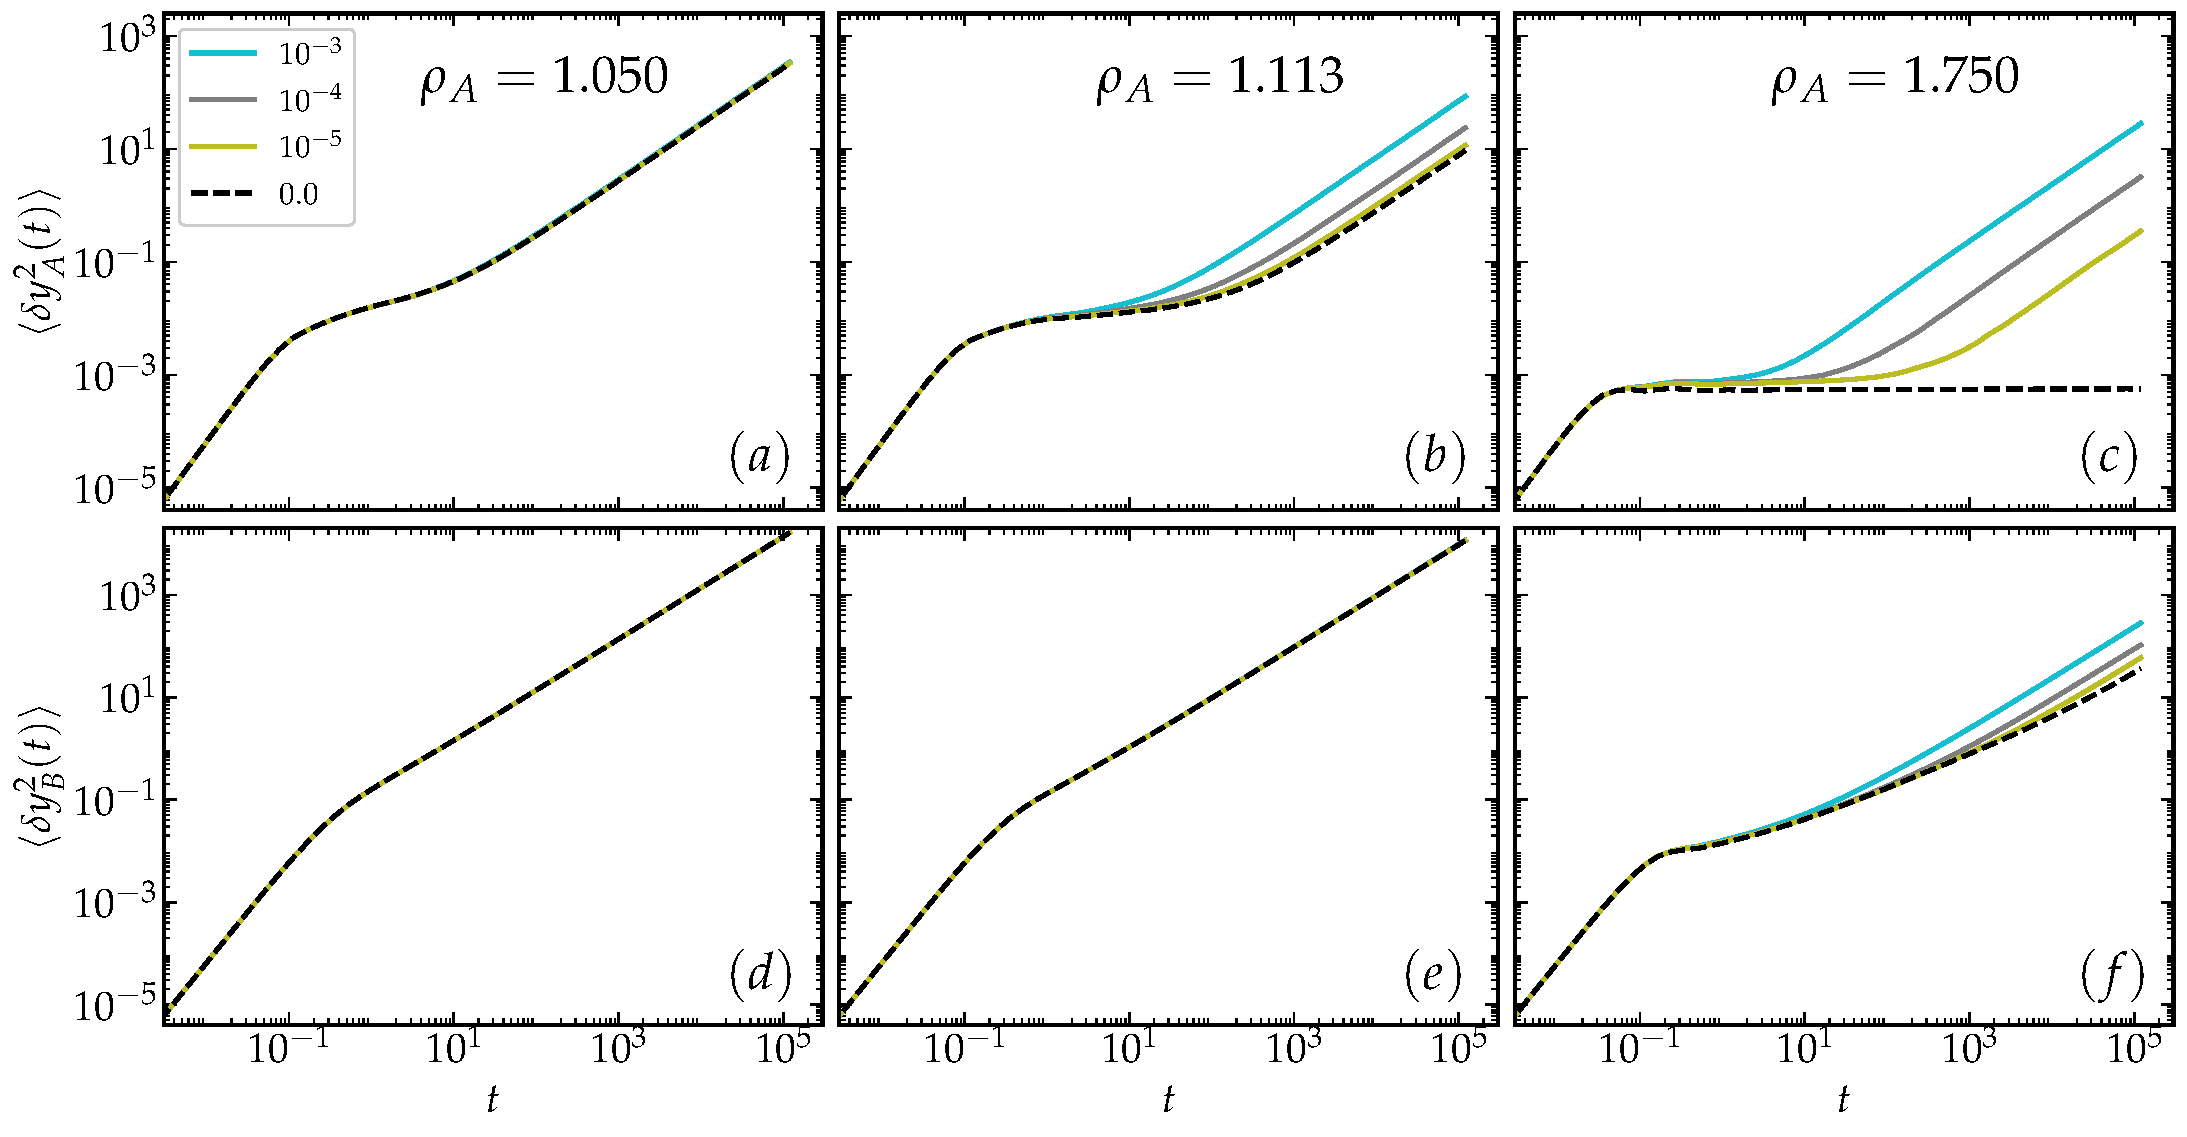
\includegraphics[width=15cm]{figs/fig7p6af.pdf}
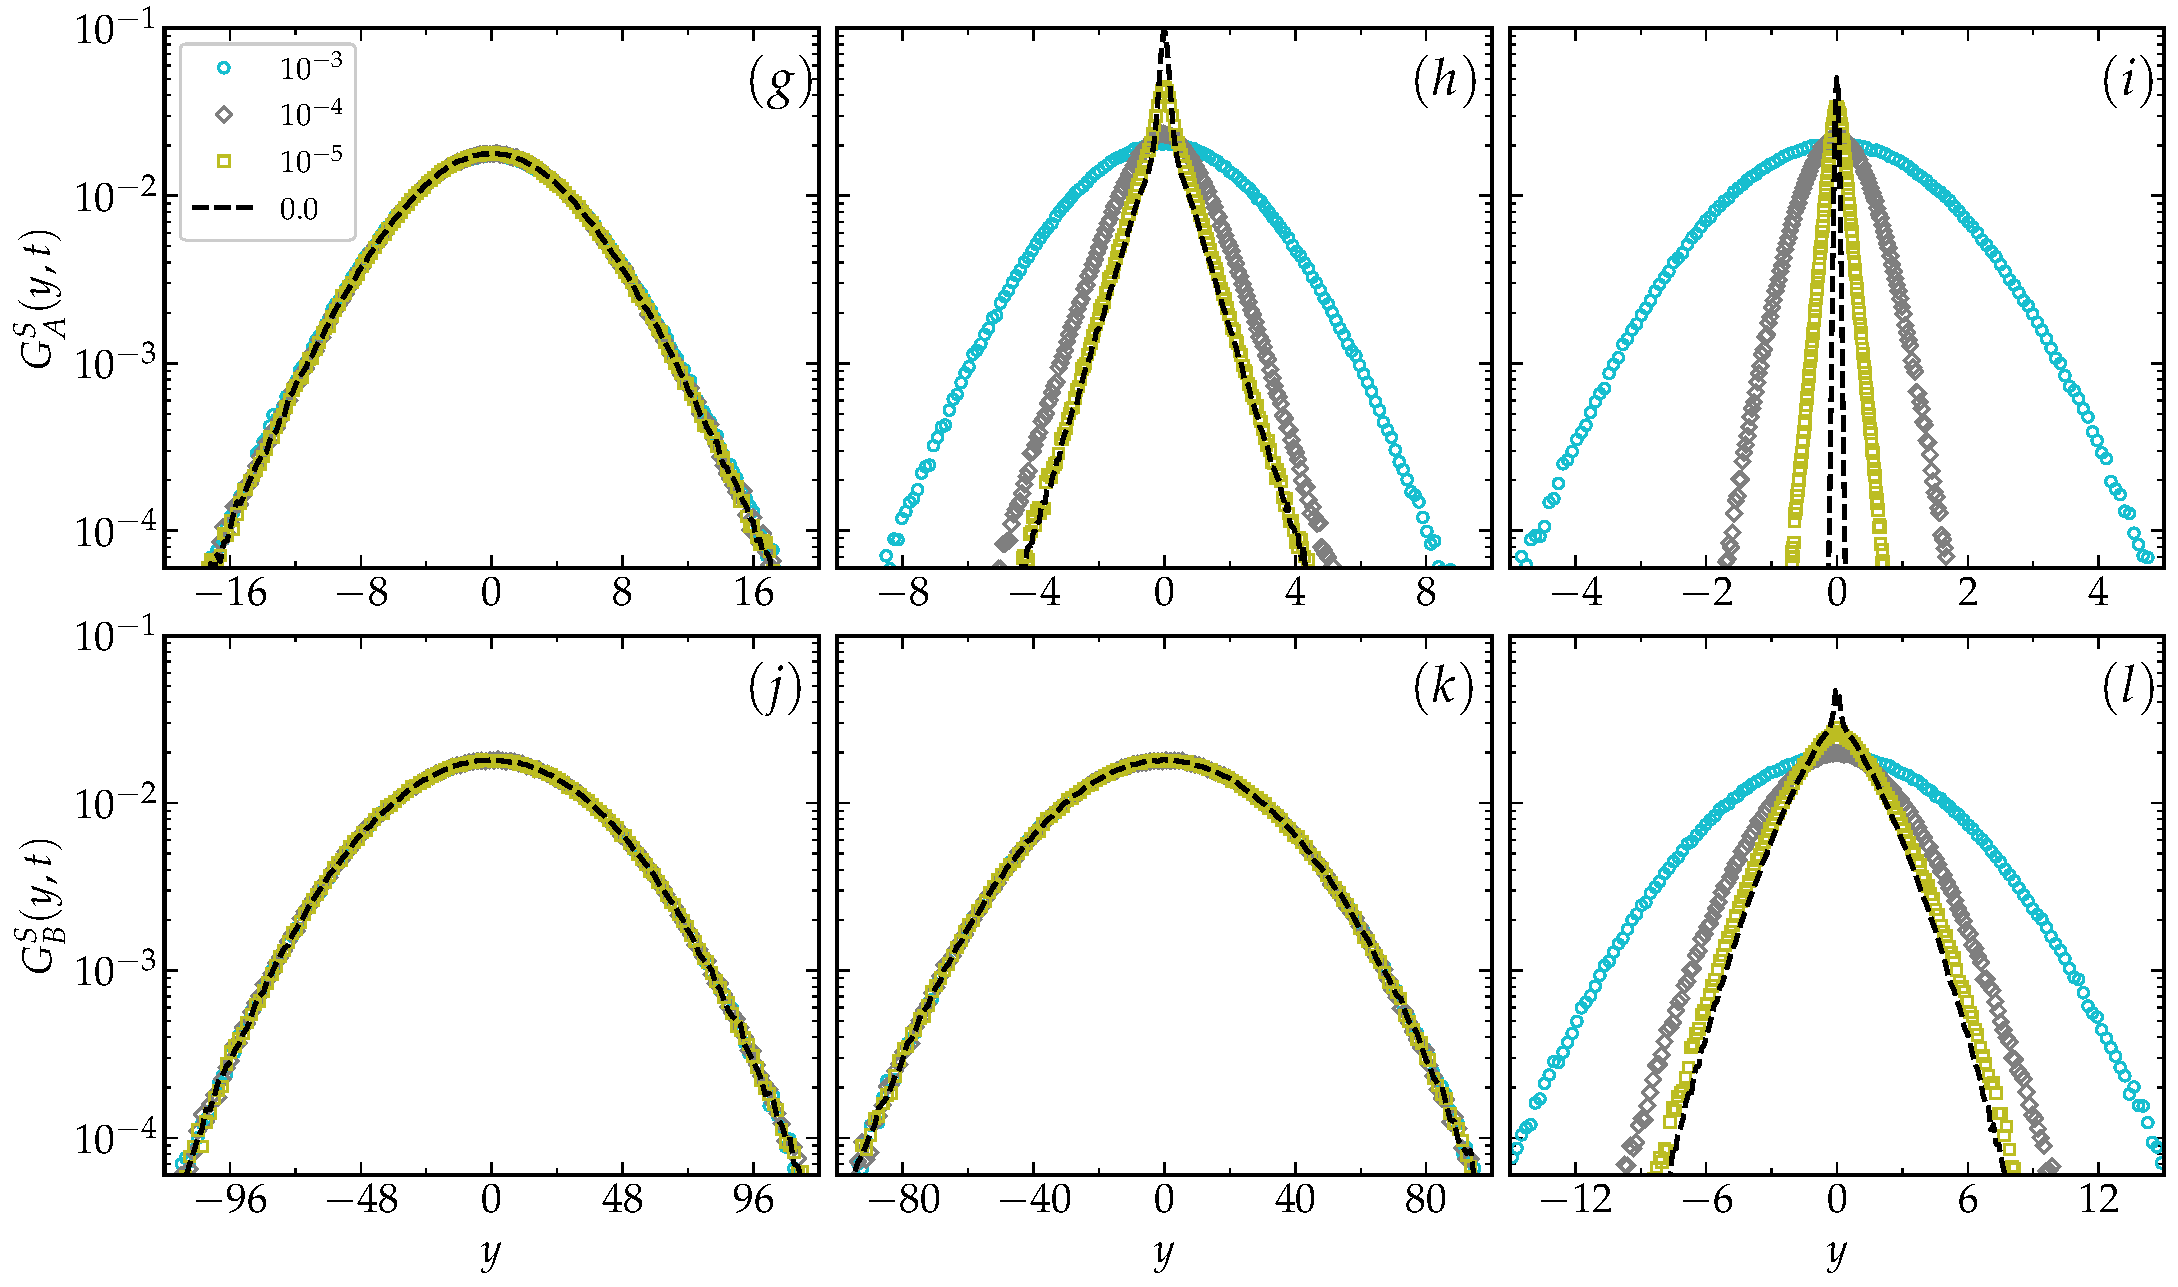
\includegraphics[width=15cm]{figs/fig7p6gl.pdf}
\caption[{\em Microscopic dynamics under applied shear: mean squared displacement and self part of van Hove function}]{{\em Microscopic dynamics under applied shear}: Mean squared displacement of bigger (a-c) and smaller (d-f) species in the presence (with solid lines) and in the absence (with dotted lines) of shear, measured in the vorticity direction. Corresponding self part of van Hove function, $G_s(y,t)$ of bigger species (g-i) and smaller (j-l) species in the presence (with symbols) and absence (dotted lines) of shear, at $t=8075.4$, also measured in the vorticity direction. In both cases, first column represents system at partial density $\rho_{\rm A} = 1.050$, middle at $\rho_{\rm A} = 1.113$ and last at $\rho_{\rm A} = 1.750$. 
\label{fig6}}
\end{figure*}
%

%
\subsubsection{Steady-state microscopic dynamics}
%
In order to further analyse the rheological response, we study the microscopic dynamics of the system in steady state. In the vorticity direction, i.e., normal to the shear plane, we compute the MSD for the A and B species, separately, as well as the self part of the van Hove function of which MSD is the second moment.  The van Hove Function, $G_s(r,t)$ is measured at a late time ($t=8075.4$) in each case. The corresponding aggregated plots showing the variation of the dynamics with changing density are shown in Fig.~\ref{fig6}, for MSD and $G_s(r,t)$, for a range of imposed shear rates. All measurements are done in the center-of-mass reference of respective species, to remove the effects resulting from finite center-of-mass diffusion in the glassy regime of A species.

At the smaller density ($\rho_{\rm A} = 1.050$), we do not observe any variation in the dynamics with imposed shear rate, for both A and B species. In both cases, the MSD curves as well as the $G_s(r,t)$ data are indistinguishable between the equilibrium and non-equilibrium regimes. This corresponds to the linear response regime, which is characterised by the Newtonian viscosity, see Fig.~\ref{fig6} (a), (d) for the MSD data and the corresponding data for $G_s(r,t)$ in Fig.~\ref{fig6} (g), (j).

If we now consider the higher density, $\rho_{\rm A} = 1.113$,  which is in the vicinity of $\rho_{\rm A}^{\rm MCT}$, we observe that for the B species, the indistinguishability between the equilibrium and non-equilibrium data for MSD and $G_s(r,t)$ continue, i.e., the external shear is having no effect; see Fig.~\ref{fig6} (e), (k). However, for the A species, the shear introduces deviation from equilibrium behaviour, with a decrease in the caging time and subsequent enhancement in long-time diffusive dynamics with increasing shear rate, as is visible in the MSD data (Fig.~\ref{fig6} (b)) which is also evident in the distinct change in the shape of the corresponding $G_s(r,t)$ (Fig.~\ref{fig6}(h)). Thus, at this density, the imposed shear rate corresponds to a timescale which is faster than the equilibrium relaxation timescale of the A species, but not for the B species. Note that, for this density, an apparent macroscopic yield stress is visible. Thus, we can conclude that the apparent emergence of macroscopic rigidity and subsequent yielding under shear is a consequence of the interplay between the external drive and the structure formed by the A species, while the B species remain oblivious to this process and thus seems inconsequential to the overall rheological response, i.e., variation of viscosity with shear rate in this density regime.

However, if we go to even larger densities, $\rho_{\rm A}=1.750$, the imposed shear affects the dynamics of both the A and B species; see Fig.~\ref{fig6} (c), (f), (i), (l); for both species, enhanced diffusion is observed with increasing shear rate. Thus, the imposed timescales via the shear are faster compared to the equilibrium relaxation timescale for both species, even though there is still a large separation in dynamical timescales in the quiescent state. We also note that for the B species, the sub-diffusive dynamics still persists, except that the time-window for subdiffusion decreases with increasing shear-rate and this timescale seems to be determined by the caging timescale of the A species under shear. Or in other words, the localization dynamics of the smaller particles within the matrix formed by the B species has a reduced lifetime due to the shear which fluidizes the matrix over a certain timescale.

%
\begin{figure}[htb!]
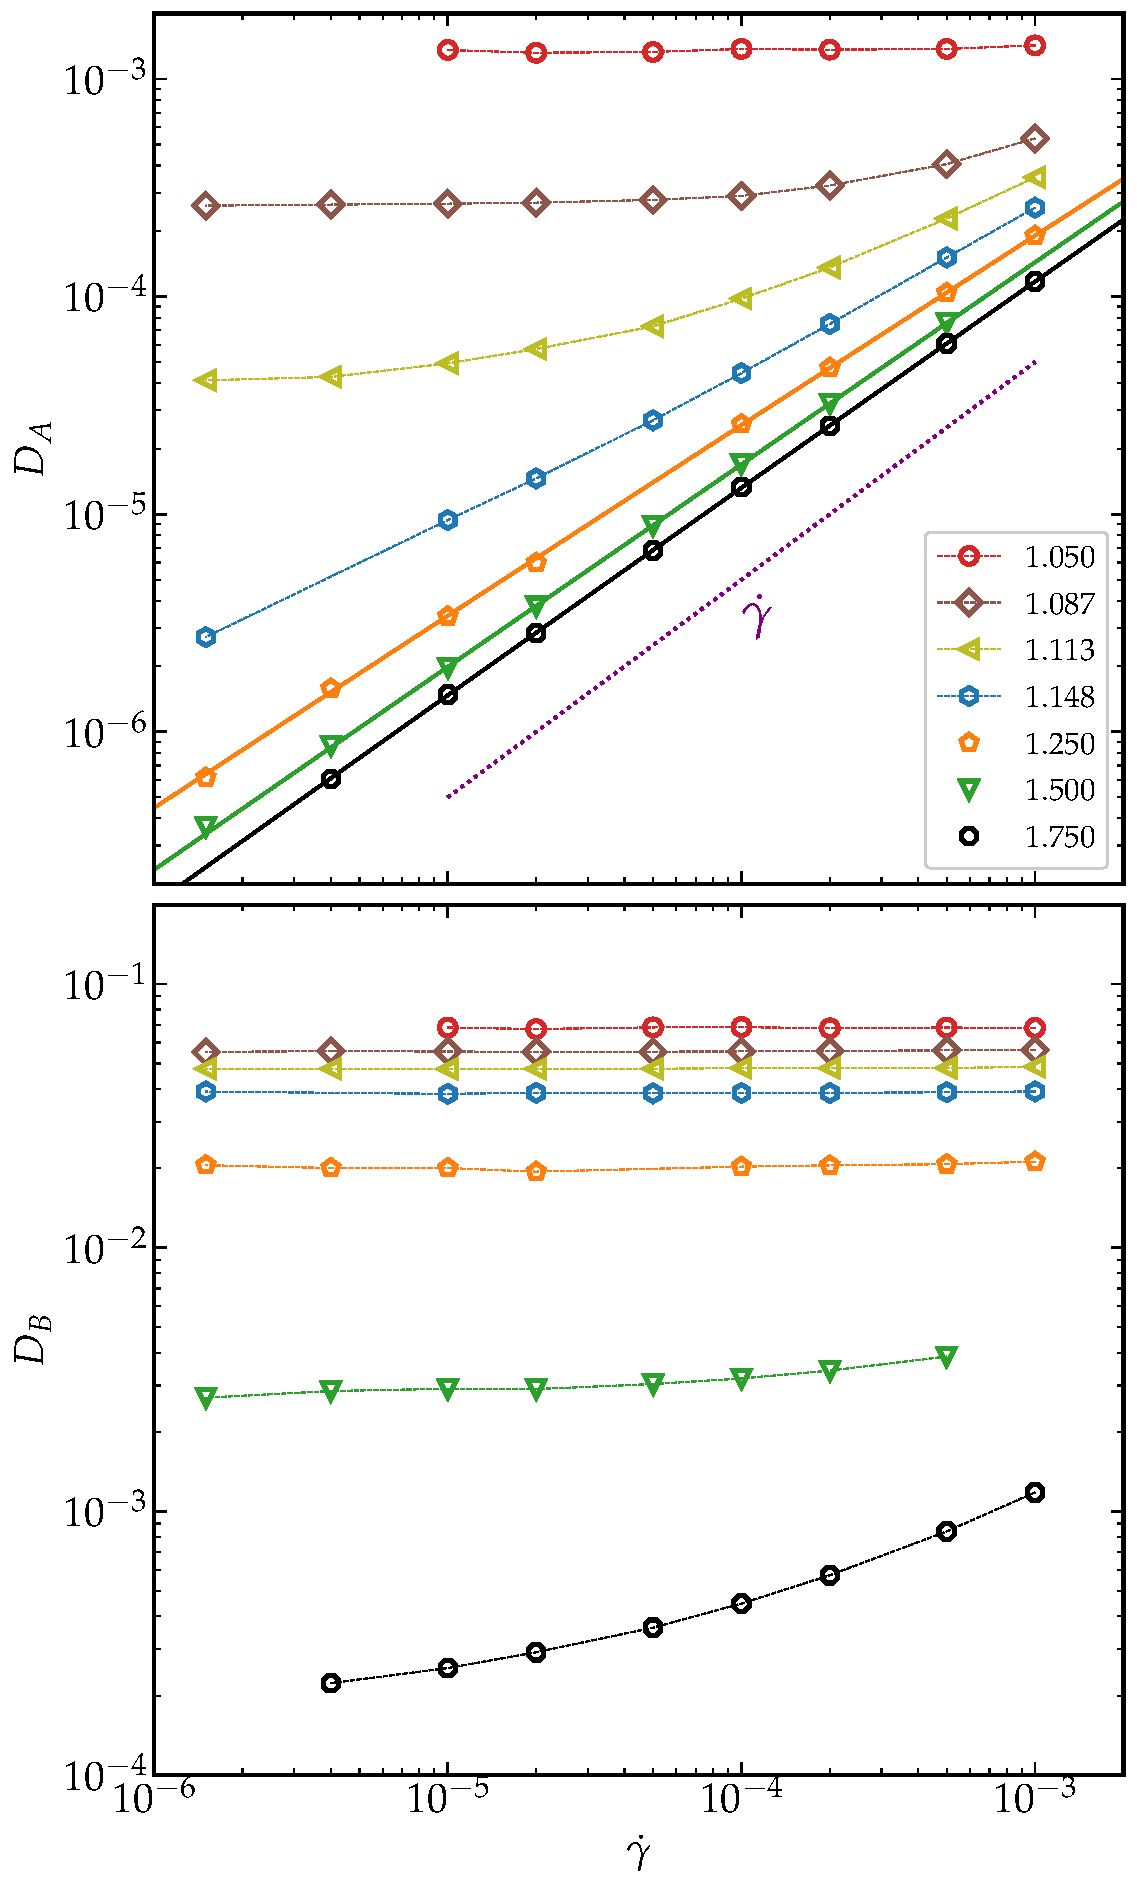
\includegraphics[width=11cm]{figs/fig7p7.pdf}
\centering
\caption[{\em Diffusion coefficient in the presence of shear}]{{\em Diffusion coefficient in the presence of shear.} Variation of diffusion coefficient of bigger (top) and smaller (bottom) species with shear rate, measured in the vorticity direction, at different partial densities of bigger species as marked. In the top panel, the solid lines correspond to fits using $C\dot{\gamma}/(1+D\dot{\gamma}^{\delta})$ (see text for discussion). The obtained fit parameters are: $C = 1.998, 1.426, 0.267$, $D = 25.943, 15.480, 2.507$ and $\delta = 0.145, 0.079, 0.097$ for $\rho_A = 1.25, 1.50, 1.75$. The dashed line corresponds to $\dot{\gamma}$, for reference}.
\label{fig7}
\end{figure}
%

We can extract a diffusion coefficient from the long-time diffusive dynamics observed in the MSD data, for the various imposed shear rates at different densities. The shear rate dependence of the diffusion constant, for the range of densities explored, is shown in Fig.~\ref{fig7}, for both A and B species.

At small densities, the diffusion coefficient for both A and B species has no shear rate dependence, which is just a reflection of the fact that the dynamics remains unaffected by the shear, as discussed above. This behaviour continues for B species up to very large densities where the shear starts to have an effect.  Also, in this density regime, the diffusion coefficient for A species has a power-law dependence on shear rate and appears to vanish at $\dot{\gamma} \rightarrow 0$, which is typical to the shear response of amorphous systems. We show that it is possible to fit the shear-rate dependence of diffusion coefficient using a generalized Stokes-Einstein form: $D_A(\dot{\gamma}) \sim 1/\eta(\dot{\gamma}) \sim C\dot{\gamma}/(1+D\dot{\gamma}^{\delta})$, using the Herschel-Bulkley form discussed earlier, with $C$, $D$ and $\delta$ being fit parameters. Note that if $D\dot{\gamma}^{\delta} << 1$, the leading order behaviour would be $\sim \dot{\gamma}$, which is what we observe as indicated in the top panel of Fig.~\ref{fig7}. In the intermediate density regime, the diffusion coefficient also decreases with decreasing shear rate, but deviates from a power-law behaviour and seems to reach a constant at vanishing shear rates. This would imply that there is a diffusive behaviour in the absence of shear at these densities. This behaviour is observed around the density where the onset of glassiness occurs for the A species, viz.~in the vicinity of $\rho_{\rm A}^{\rm MCT}$. We also note that for B species a similar behaviour is observed at the largest density that we have explored, implying that in the absence of shear, the smaller particles would be undergoing equilibrium diffusive dynamics in that density regime.

To summarise, from the rheological response of the binary mixture, we infer that beyond $\rho_{\rm A}^{\rm MCT}$, an apparent yield stress emerges which is linked to the glassiness undergone by the A species. On contrary, the B species continue to be very mobile inside the matrix formed by the A species and their dynamics does not couple to the shear, and thus their contribution to the system's shear response is minimal. Only at much higher densities, the yielding process involves the collective interplay of both A and B species.

%
\begin{figure}[htb!]
\centering
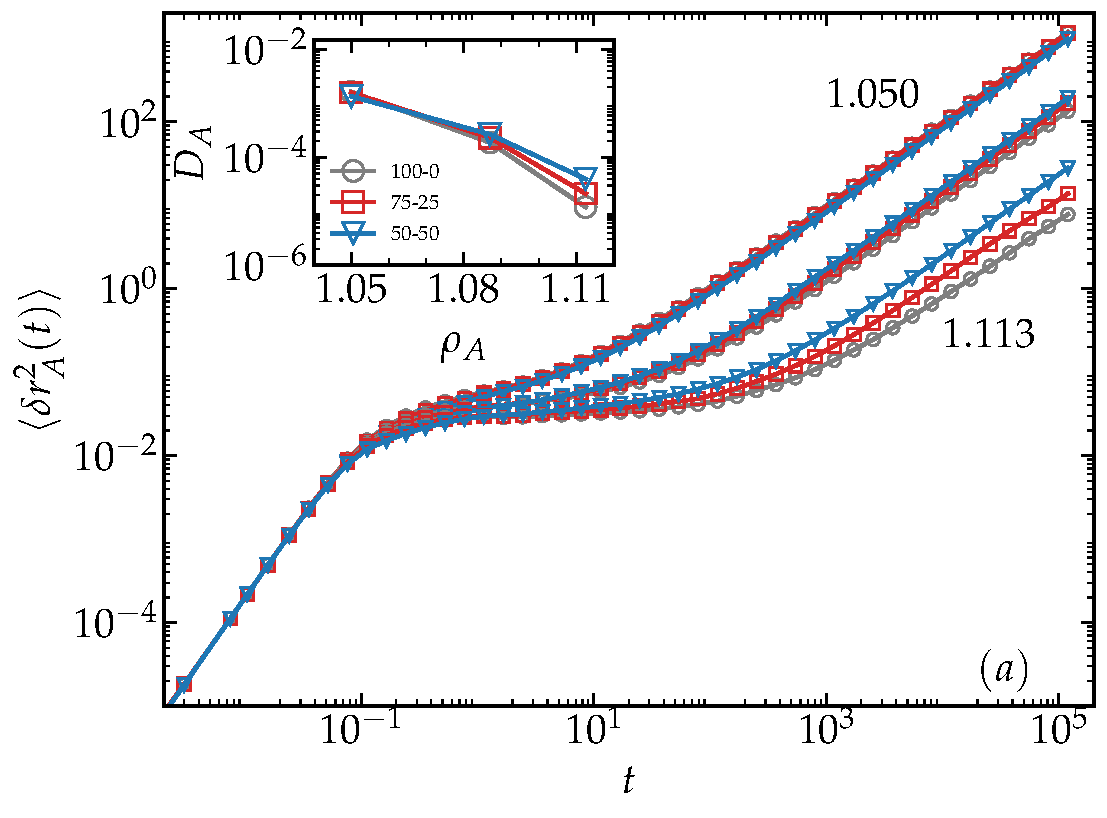
\includegraphics[width=7.5cm]{figs/fig7p8a.pdf}
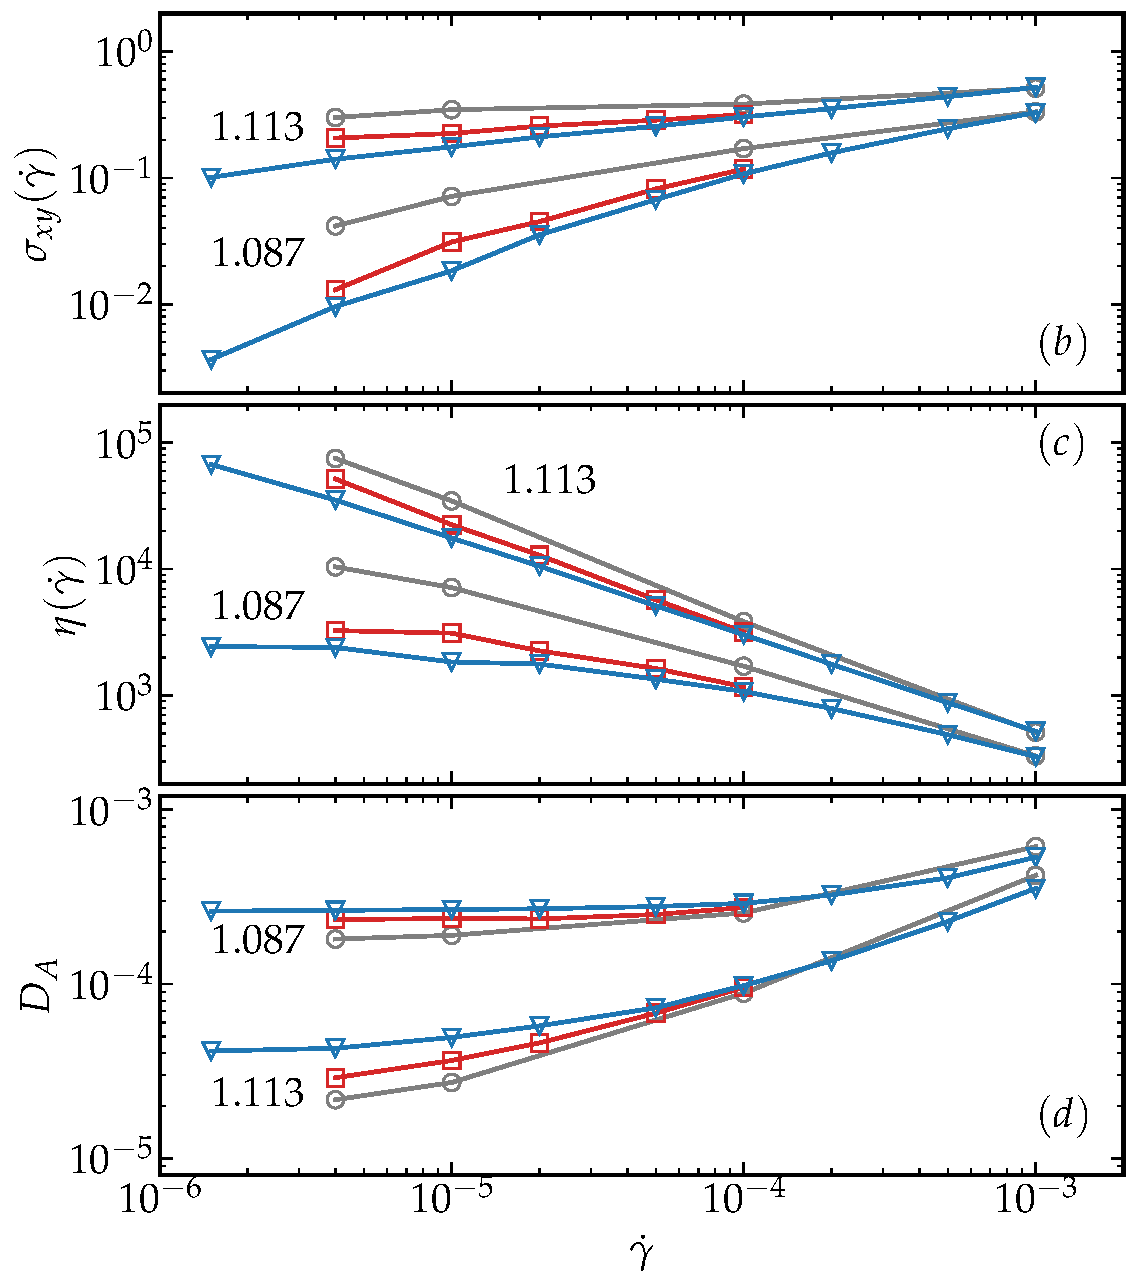
\includegraphics[width=7.5cm]{figs/fig7p8bd.pdf}
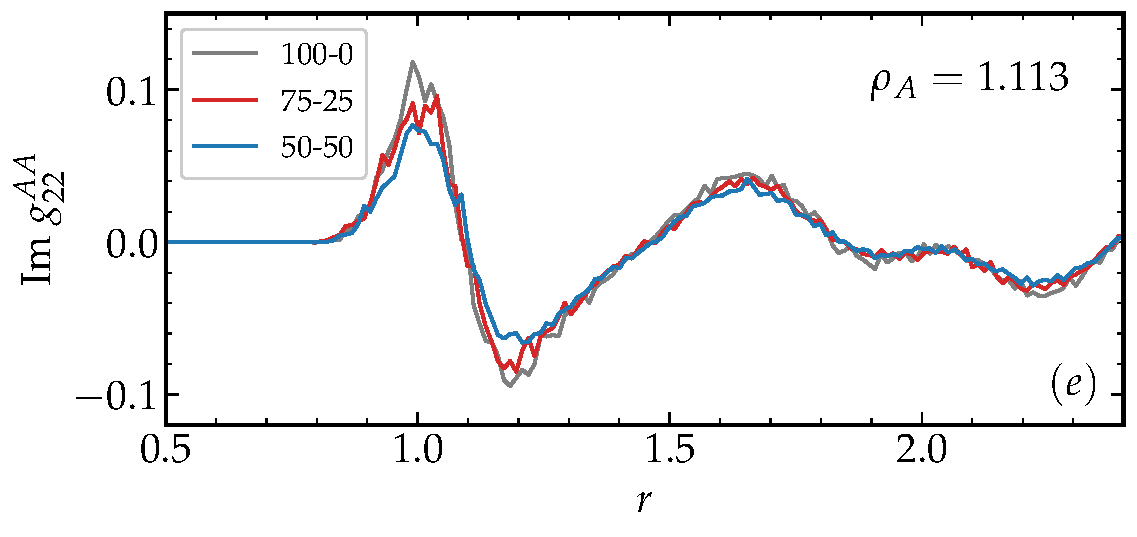
\includegraphics[width=7.5cm]{figs/fig7p8e.pdf}
\caption[{\em Effect of varying composition in quiescent and sheared samples}]{{\em Effect of varying composition}. (a) {\em  Quiescent behavior.} MSD measured for the A species, for different composition of the mixture (circle: 100-0, square: 75-25, triangle: 50-50). (Inset) Variation of larger particle diffusion coefficient with partial density $\rho_{\rm A}$ for different composition of the system. (b-d) {\em Rheological response.} Shear stress and viscosity as a function of shear rate for different composition of the mixture. And, diffusion coefficient versus shear rate for the same compositions. (e) The function ${\rm Im} \, g_{22}^{\rm AA}(r)$ for the different compositions at the partial density $\rho_{\rm A}= 1.113$ and shear rate $10^{-4}$.} \label{fig8}
\end{figure}
%

%
\subsubsection{Role of smaller species: varying the composition}
%
We now address the question of what role do the B species play in the rheological response.  We address this questions by varying the composition of the mixture, and even considering the situation where the B species are completely absent.

We begin by first examining how the equilibrium behaviour of the system is influenced by the presence or absence of the B species. In Fig.~\ref{fig8}(a), we show the MSD data for the A species for varying A:B compositions, viz.~100:0, 75:25 and 50:50 for three different $\rho_{\rm A}$. We note that at small densities, there is no variation in the dynamics, but at relatively larger densities ($\rho_{\rm A} = 1.113$) there is distinct variation with the long-time dynamics becoming faster with increased presence of B species. This is also reflected in the measured diffusion coefficients as shown in the inset of Fig.~\ref{fig8}(a). From this data, it would imply that $\rho_{\rm A}^{\rm MCT}$ shifts to larger densities with the increasing inclusion of B species. This would be consistent with previous findings in other soft glassy systems, e.g. asymmetric star polymer mixtures, \cite{zaccarelli2005}, where insertion of a population of smaller particles led to the melting of the glass formed by the larger particles. It is also interesting to note that, the insertion of the smaller species has a very different effect than insertion of bigger particles in a system of smaller particles. In the latter case, the bigger particles act as pinning sites and slow down the dynamics.

Next, we study how the rheological response changes, in the presence or absence of the small particles. In Fig.~\ref{fig8}(b),(c),(d), we do a comparison of the rheological curves as well as the microscopic dynamics for the different compositions listed above. The effect of enhancement in equilibrium dynamics due to the presence of B species is reflected in the rheology data, especially in the intermediate density regime (as the glassy regime of A species is approached), where the viscosity of the system distinctly decreases at small shear rates with increasing presence of B species. This effect is absent at small densities and also at very large densities where the entire system becomes glassy. Thus, in the intermediate density regime, the mobile B population does have a softening effect on the overall shear response, an effect which can be exploited in various applications.

It is also interesting to relate the change of the shear stress with composition to the spatial information provided by ${\rm Im} \, g_{22}^{\rm AA}(r)$. In Fig.~\ref{fig8}(e), this function is shown for the different compositions at the partial density $\rho_{\rm A}= 1.113$. Obviously, significant  changes in ${\rm Im} \, g_{22}^{\rm AA}(r)$ due to changes in composition are only seen for distances $r<1.5$ where this function exhibits an oscillation with a peak around $r=1.0$ and a negative dip around $r=1.2$ (cf.~Fig.~\ref{fig5}). From this behavior of ${\rm Im} \, g_{22}^{\rm AA}(r)$, we can infer that compositional changes in the anisotropies due to shear occur on local length scales $r<1.5$.

Our findings are consistent with experiments involving colloidal glasses with constituents having large size ratio, where a similar softening of the material was observed with increasing insertion of small particles till a 50:50 composition was reached \cite{sentjabrskaja18, sentjabrskaja19}.

%
\section{Conclusions}
%
Our work on the quiescent dynamics elucidates several aspects of the diffusion dynamics in an equimolar glassforming binary soft-sphere mixture with large size ratio.  We observe a very pronounced time scale separation between the motion of the slow A species and that of the fast B species at high densities. As a consequence, the A particles show the typical glassy dynamics of a densely packed system, while the B particles remain mobile at very high densities, $\rho > \rho_c$, exploring the void space in between the A particles. We have seen that the interdiffusion coefficient $D_{\rm AB}$ can be well approximated by the Darken equation (\ref{eq_darken}).  Since at high density $D_{\rm A} \ll D_{\rm B}$, one therefore obtains $D_{\rm AB} \approx \Phi x_{\rm A} D_{\rm B}$, i.e.~the interdiffusion coefficient is dominated by the fast species.  For our equimolar mixture, we can also write $D_{\rm AB} = \Phi N D_{\rm A}^{\rm cm}$ and thus at high density we have $D_{\rm A}^{\rm cm} \approx D_{\rm B}/(2N)$.  This implies that even if the A particles form a frozen-in structure with essentially no rearrangements of the relative positions of particles, they may follow collectively the diffusive motion of their center of mass and one finds for the selfdiffusion coefficient $D_{\rm A} \approx D_{\rm A}^{\rm cm} \propto N^{-1}$. One can, of course, correct for this finite-size effect by computing one-particle quantities such as MSD$_{\rm A}(t)$ and $F_s^{\rm A}(q,t)$ from the center-of-mass-corrected coordinates, as defined above.

The finite-size effects, that we have reported here with respect to the selfdiffusion coefficient of the slow species, are expected to be a typical feature in glassforming binary mixtures with large size ratio. Moreover, one may expect similar effects in any glassforming system with strong dynamic heterogeneities. {Furthermore, studying interdiffusion dynamics with changing composition as well as size-ratio of the mixture would be of interest, since variation of these parameters are known to change extensively the dynamical properties of the mixture \cite{zac2005, vinaySoft}}.

In the context of our study on the rheological response reported in this chapter, the main observation comes via the measured shear stress, in steady state, as a function of the imposed shear rate. At small densities, the low shear rate regime corresponds to that of a Newtonian fluid. However, in the density regime where the larger species within the mixture undergo a mode coupling dynamical transition in the quiescent state, the shape of the flow curves change at vanishing shear rates and an effective yield stress can clearly be estimated. Thus, there is a macroscopic rigidity. If we now focus on the microscopic dynamics, we observe that while the motion of the larger species indeed get influenced by the external shear, the dynamics of the smaller species remain completely unchanged vis-a-vis their motion in the absence of shear, within the explored range of shear rates. Thus, the macroscopic rigidity at vanishing shear rate is occurring while there is a highly mobile population of the smaller species within the system.

With increasing density, the yield stress increases as expected and the diffusion coefficient of the larger species exhibit a distinct power-law behaviour as a function of applied shear rate which is a distinctive feature of glassy systems. Only at large densities, we start to observe that the external shear rate is able to influence the motion of the smaller species, i.e., the timescale imposed by the applied shear rate is large enough to compete with the relaxation timescale of the smaller species.

To better understand the rheological behaviour of the mixture, we provide a structural analysis by quantifying the developing anisotropies due to the imposed shear. The main finding of this analysis is that the dominant contribution to the stress comes from the correlations between the large particles, which therefore is the main source of the emergent rigidity within the system as density is increased. The other correlations, viz. that between the smaller particles and the cross-correlation between the two species are much smaller in magnitude. Interestingly, it turns out that the nature of the cross-correlation is such that the contribution to the stress is negative. Whether this can be tuned by varying the particle interactions as well as composition of the mixture, such that the rheological behaviour is affected, needs to be explored in future.

Finally, we have probed the role of the smaller species in the rheological response of the mixture, since the macroscopic rigidity emerges in the system even though these particles remain highly mobile. We observe that if we start with a system of just the large particles and then start inserting the smaller species, i.e., systematically change the mixture's composition, the rheological response changes in the small shear rate regime, viz.~the viscosity of the system decreases. Thus, the presence of the smaller particles softens the mixture's mechanical response, which is consistent with experimental observation in similar colloidal mixtures. Note that similar plasticizing effects have also been reported for polymeric systems \cite{zaccarelli2005, kalathiprl2012} where the inclusion of very small colloidal particles led to softening. Hence, this indicates to a very generic mechanism at play in how such inclusions can influence rheology.  We also note here that this behaviour is in contrast to the situation where the inclusion of large particles in a matrix of small particles can lead to hardening of the system, i.e., the rheological behaviour of the mixture changes as the composition is changed.
